%  LaTeX support: latex@mdpi.com 
%=================================================================
\documentclass[electronics,article,submit,pdftex,moreauthors]{Definitions/mdpi} 

%=================================================================
\firstpage{1} 
\makeatletter 
\setcounter{page}{\@firstpage} 
\makeatother
\pubvolume{1}
\issuenum{1}
\articlenumber{0}
\pubyear{2026}
\copyrightyear{2026}
\datereceived{ } 
\daterevised{ } 
\dateaccepted{ } 
\datepublished{ } 
	extit{Increasing Teacher Effectiveness}, 2nd~ed.;

\usepackage{multirow}
\usepackage{booktabs}
\usepackage[ruled,lined,linesnumbered]{algorithm2e}
\usepackage{tikz}
	extit{Educ. Inf. Technol.} \textbf{2023}, \textit{28}, 7127--7155.
\crefname{algocf}{Algorithm}{Algorithms}
\Crefname{algocf}{Algorithm}{Algorithms}
\graphicspath{{figures/}}

In \textit{Proceedings of the 38th International Conference on Machine Learning}; Virtual, 18--24 July 2021; pp.~8748--8763.
\Title{Benchmarking CLIP-Family Models for Zero-Shot Classroom Activity Recognition: Prompt and Metric Choice Matter}

\Author{Yan Ma $^{1,3}$ and Lizhuo Zhang $^{2,}$*}

	extit{Adv. Neural Inf. Process. Syst.} \textbf{2022}, \textit{35}, 25278--25294.

\address{%
$^{1}$ \quad School of Education, Hunan Agricultural University, Changsha 410128, China\\
$^{2}$ \quad School of Information and Intelligence, Hunan Agricultural University, Changsha 410128, China; zhanglizhuo@hunau.edu.cn\\
	extit{arXiv} \textbf{2025}, arXiv:2502.14786.

\corres{Correspondence: zhanglizhuo@hunau.edu.cn}

\simplesumm{}
	extit{arXiv} \textbf{2023}, arXiv:2303.11331.
%=================================================================
\abstract{%
This paper presents a benchmark study of zero-shot classroom activity recognition using CLIP-family vision--language models as \emph{probes}, with prompt choice and metric choice treated as first-order experimental variables rather than reporting details. The probes are deployed under a multi-scene benchmark built from three public SCB subsets: TeacherBehavior (8 classes, 3240 validation images, multi-label), HandriseReadWrite (3 classes, 1671 images), and BowTurnHead (2 classes, 505 images); five ViT-Large backbones (CLIP/OpenAI, OpenCLIP/LAION, SigLIP2, EVA02-CLIP, DFN-CLIP) are evaluated together with four uniform prompt strategies and a training-free class-aware prompt ensemble, CAPE. The headline finding is that \emph{prompt design dominates over backbone choice}: action prompts improve TeacherBehavior Hit@1 by up to 54 percentage points over label-only prompts, and CAPE robustness is itself prompt-wording-sensitive (e.g., on SigLIP2, alternate-wording Set~B drops Hit@1 from 95.5\% to 31.4\% on TeacherBehavior). CAPE is effective but task-dependent rather than universally optimal: it leads on TeacherBehavior (85.56\%, SigLIP2) and on BowTurnHead (a nominal 93.27\% multi-label Hit@1 with DFN-CLIP, only $\sim$2.6~pp above the multi-label majority floor of 90.69\% on that 2-class subset and therefore best read as a small effect on top of a near-saturated lenient metric), whereas a simpler action prompt is best on HandriseReadWrite (84.56\%, OpenCLIP). Evaluation protocol substantially changes conclusions: under non-oracle multi-label thresholding, supervised linear probes on frozen features reach Sample-F1 88--90\%, Macro-F1 68--78\%, and Micro-F1 89--91\% on TeacherBehavior, versus 60--66\%, 49--61\%, and 61--70\% for zero-shot CAPE---i.e., the zero-shot Hit@1 advantage is largely a lenient-metric artifact. Bootstrap confidence intervals (1000 resamples) and paired-bootstrap significance tests further show that several headline gaps lack hypothesis-tested support. Cross-family checks against three MLLMs and an EVA02 CAPE-vs.-best-prompt comparison reinforce that classroom zero-shot benchmarks should report multiple metrics, prompt strategy, and uncertainty estimates alongside headline Hit@1.%
}
	extit{arXiv} \textbf{2023}, arXiv:2309.17425.
\keyword{zero-shot classification; CLIP; classroom activity recognition; prompt engineering; vision--language models; multi-scene benchmark; EVA-CLIP; teacher behavior analysis}

%%%%%%%%%%%%%%%%%%%%%%%%%%%%%%%%%%%%%%%%%%
\begin{document}
	extit{IEEE Trans. Affect. Comput.} \textbf{2014}, \textit{5}, 86--98. doi:10.1109/TAFFC.2014.2316163.
%=================================================================
% 1. Introduction
%=================================================================
\section{Introduction}
In \textit{Proceedings of the 7th International Learning Analytics \& Knowledge Conference (LAK)}; Vancouver, BC, Canada, 13--17 March 2017; pp.~218--227. doi:10.1145/3027385.3027400.

Automatic recognition of classroom teaching activities is essential for educational quality assessment, teacher professional development, and intelligent classroom analytics~\cite{brophy2000teaching,anderson2004classroom}.
In modern smart classrooms, camera systems continuously capture teaching and learning behaviors for downstream analysis~\cite{dillenbourg2011classroom}.
Developing robust image-based recognition pipelines---especially ones that require no task-specific training data---is a key enabler for scalable educational AI.
Traditional approaches rely on supervised deep learning models that require large-scale labeled training data, which is expensive and time-consuming to collect in real classroom environments~\cite{liu2023survey_classroom}.

Vision--language foundation models, exemplified by CLIP (Contrastive Language--Image Pretraining)~\cite{radford2021learning}, have recently emerged as powerful tools for zero-shot visual recognition.
By learning joint image--text representations from web-scale data, CLIP enables classification without any task-specific training---users simply provide natural language descriptions of target categories.
Several CLIP variants have since been proposed, including OpenCLIP trained on LAION-2B~\cite{schuhmann2022laion5b}, SigLIP2~\cite{tschannen2025siglip2}, EVA02-CLIP~\cite{sun2023eva02}, and DFN-CLIP~\cite{fang2023data}, each offering different training objectives, data curation strategies, or architectural innovations.
	extit{J. Educ. Comput. Res.} \textbf{2020}, \textit{58}, 63--86. doi:10.1177/0735633119825575.
Despite their success on general benchmarks, the applicability of CLIP-family models to fine-grained classroom activity recognition remains largely unexplored.
Classroom activities present unique challenges: visually similar actions (e.g., ``standing'' vs.\ ``teaching''), domain-specific semantics, significant class imbalance, and inherent \emph{multi-label} structure---a single classroom image typically contains multiple concurrent activities (e.g., a teacher simultaneously lecturing, standing, and referencing a screen).
Moreover, different classroom scenes---teacher lecturing, student individual learning, subtle micro-actions, and group discussion---pose qualitatively different recognition demands that a single dataset cannot capture.
The \emph{prompt design}---how activity categories are described in natural language---can substantially affect zero-shot performance, yet systematic studies of prompt strategies for educational scenarios are scarce.
	extit{Front. Psychol.} \textbf{2022}, \textit{13}, 903560. doi:10.3389/fpsyg.2022.903560.
In this study, CLIP-family models are used primarily as \emph{probes} rather than as the main methodological contribution. The main objective is to determine how prompt choice, metric choice, and backbone family change the conclusions drawn from zero-shot classroom benchmarks. Specifically, the analysis tests whether headline results remain stable once prompt wording is varied, class-balanced multi-label metrics are emphasized alongside lenient Hit@1, and multiple CLIP-family backbones are compared under a common protocol; it also examines whether TeacherBehavior remains the hardest subset because it contains semantically overlapping categories and stronger context dependence, whereas BowTurnHead and HandriseReadWrite are comparatively easier due to clearer visual boundaries.

This study addresses these gaps with six contributions:

In \textit{Proceedings of the IEEE/CVF Conference on Computer Vision and Pattern Recognition (CVPR)}; Vancouver, BC, Canada, 18--22 June 2023; pp.~2818--2829. doi:10.1109/CVPR52729.2023.00276.
    \item \textbf{Multi-scene benchmark.} A classroom activity benchmark is constructed by integrating three publicly available SCB sub-datasets spanning teacher behavior, student learning actions, and negative micro-actions, covering 13 activity categories across 5416 validation images.
    
    \item \textbf{Probe-based cross-model analysis.} Five representative CLIP-family models (CLIP-OpenAI, OpenCLIP-LAION, SigLIP2, EVA02-CLIP, and DFN-CLIP), all at the ViT-Large scale, are benchmarked under a unified classroom zero-shot protocol and interpreted as analysis probes for task difficulty rather than as competing method proposals.
    
In \textit{Proceedings of the IEEE/CVF International Conference on Computer Vision (ICCV)}; Paris, France, 2--6 October 2023; pp.~11975--11986. doi:10.1109/ICCV51070.2023.01100.
    
    \item \textbf{Prompt choice matters more than backbone choice in several settings.} CAPE is treated here as one prompt strategy rather than the paper's primary contribution. The results show that it is \emph{not} universally optimal: it excels on semantically ambiguous tasks (teacher behavior, micro-actions) but is outperformed by simple action prompts when class boundaries are visually well-separated (student learning actions). This task dependency provides guidance for prompt strategy selection.
    
    \item \textbf{Stable difficulty hierarchy evidence.} Across prompts and backbones, the results repeatedly indicate a difficulty ordering in which TeacherBehavior is hardest, HandriseReadWrite is intermediate, and BowTurnHead is comparatively easier, supporting the view that classroom-task difficulty is an intrinsic property rather than a single-model artifact.
In \textit{Proceedings of the 2022 Conference on Empirical Methods in Natural Language Processing (EMNLP)}; Abu Dhabi, United Arab Emirates, 7--11 December 2022; pp.~3876--3887. doi:10.18653/v1/2022.emnlp-main.256.
    \item \textbf{Metric-sensitive and reproducible benchmark analysis.} Cross-family analyses using MLLM references and a direct comparison between EVA02 under CAPE and EVA02 under its best prompt strategy show that class-balanced metrics and reproducibility checks materially affect the interpretation of several headline zero-shot results.
\end{enumerate}

\begin{figure}[H]
	extit{IEEE Trans. Geosci. Remote Sens.} \textbf{2024}, \textit{62}, 1--16. doi:10.1109/TGRS.2024.3390838.
\resizebox{0.98\linewidth}{!}{%
\begin{tikzpicture}[
    box/.style={rectangle, draw=black!80, line width=0.75pt, rounded corners=3.5pt,
                minimum height=0.90cm, text centered, align=center,
	extit{arXiv} \textbf{2021}, arXiv:2109.08472.
    data/.style={box, fill=blue!10},
    model/.style={box, fill=orange!14},
    proc/.style={box, fill=green!12, text width=3.05cm},
    result/.style={box, fill=red!10, text width=3.00cm},
	extit{Int. J. Comput. Vis.} \textbf{2022}, \textit{130}, 2337--2348. doi:10.1007/s11263-022-01653-1.
    stagelabel/.style={font=\scriptsize\bfseries, text=black!70,
                       rounded corners=2pt, inner sep=1.5pt}
]

In \textit{Proceedings of the IEEE/CVF Conference on Computer Vision and Pattern Recognition (CVPR)}; New Orleans, LA, USA, 18--24 June 2022; pp.~16816--16825. doi:10.1109/CVPR52688.2022.01631.
\fill[blue!4,   rounded corners=5pt] (-3.85,  0.76) rectangle (8.10, -0.72);
\fill[orange!5, rounded corners=5pt] (-3.85, -1.08) rectangle (8.10, -3.30);
\fill[green!5,  rounded corners=5pt] (-3.85, -3.55) rectangle (8.10, -6.10);
\fill[red!5,    rounded corners=5pt] (-0.45, -6.50) rectangle (10.50, -9.05);
In \textit{Proceedings of the IEEE/CVF International Conference on Computer Vision (ICCV)}; Paris, France, 2--6 October 2023; pp.~15645--15655. doi:10.1109/ICCV51070.2023.01438.
\node[stagelabel, anchor=east] at ( 7.90,  0.55) {Input Scenes};
\node[stagelabel, anchor=east] at ( 7.90, -1.30) {Feature Encoding};
\node[stagelabel, anchor=east] at ( 7.90, -3.75) {Class Prototypes \& Similarity};
\node[stagelabel, anchor=east] at (10.30, -6.70) {Evaluation Outputs};
In \textit{Proceedings of the IEEE/CVF International Conference on Computer Vision (ICCV)}; Paris, France, 2--6 October 2023; pp.~15700--15711. doi:10.1109/ICCV51070.2023.01443.
% Row 1: datasets (centered around x = 2.50)
\node[data] at (-1.00, 0.00) (ds1) {TeacherBehavior\\(8 classes)};
SCB-Dataset: Smart Classroom Behavior Dataset.
Available online: \url{https://huggingface.co/datasets/wintonYF/SCB-Dataset} (accessed on 27 April 2026).

% Row 2: image encoder (right) + prompt strategies (left)
\node[model] at ( 2.50, -1.95) (imgenc) {Image Encoder $f_{\text{img}}$\\(ViT-Large backbone)};
\node[font=\scriptsize, text=black!60] at (2.50, -2.85) (modlabel)
    {CLIP / OpenCLIP / SigLIP2 / EVA02 / DFN};
\node[proc] at (-2.20, -1.95) (prompts)
    {Prompt strategy\\\textsc{label} / \textsc{template} / \textsc{action} /\\\textsc{detailed} / \textsc{cape}};

% Row 3: text encoder, CAPE averaging, cosine similarity
\node[model] at (-2.20, -3.85) (txtenc) {Text Encoder $f_{\text{text}}$};
\node[proc]  at (-2.20, -5.40) (cape)
    {\textsc{cape}: per-class prompt averaging\\$\mathbf{t}_c = \frac{1}{|P_c|}\sum_{p\in P_c} f_{\text{text}}(p)$};
\node[proc]  at ( 2.50, -4.85) (sim)
    {Cosine similarity\\$\mathrm{sim}(\mathbf{v},\mathbf{t}_c)$};

% Row 4: outputs
\node[result] at ( 2.50, -7.10) (pred) {$\hat{y}=\arg\max_{c}\;\mathrm{sim}(\mathbf{v},\mathbf{t}_c)$};
\node[result] at ( 2.50, -8.50) (metrics) {Hit@1 / Hit@3 / Macro-F1\\Sample-F1 / Micro-F1 (Teacher)};
\node[result, text width=3.45cm] at ( 8.00, -8.50) (xcf)
    {Cross-family \& cross-prompt\\validation (MLLM, EVA02 best-prompt)};

% Arrows
\draw[arr] (ds1.south) -- ++(0,-0.30) -| (imgenc.north);
\draw[arr] (ds2.south) -- (imgenc.north);
\draw[arr] (ds3.south) -- ++(0,-0.30) -| (imgenc.north);

\draw[arr] (imgenc.south) -- node[right, font=\scriptsize]{$\mathbf{v}$} (sim.north);

\draw[arr] (prompts.south) -- (txtenc.north);
\draw[arr] (txtenc.east) to[out=0, in=180] (sim.west);
\draw[arr] (txtenc.south) -- (cape.north);
\draw[arr] (cape.east) to[out=0, in=205] (sim.west);

\draw[arr] (sim.south) -- (pred.north);
\draw[arr] (pred.south) -- (metrics.north);
\draw[arr] (metrics.east) -- (xcf.west);
\end{tikzpicture}%
}
\caption{Overview of the evaluation pipeline. Classroom images from three public SCB sub-datasets are encoded by one of five CLIP-family vision encoders to obtain image features $\mathbf{v}$. On the text side, one of five prompt strategies is applied. For the four single-prompt strategies (\textsc{label} / \textsc{template} / \textsc{action} / \textsc{detailed}), the class prototype $\mathbf{t}_c$ is the text encoding of the single prompt $p_c$. For the \textsc{cape} strategy, $\mathbf{t}_c$ is the mean of the text encodings of the three class-aware prompts in $P_c$; the dashed-style branch through the \textsc{cape} block is therefore one of the five prompt strategies, not an additional module. Classification uses cosine similarity followed by argmax; evaluation reports Hit@1/Hit@3 and multi-label F1 metrics on TeacherBehavior. Cross-family and cross-prompt validation (\Cref{sec:e11_ex}) extends the analysis with MLLM references and an EVA02 best-prompt comparison.}
\label{fig:framework}
\end{figure}


%=================================================================
% 2. Related Work
%=================================================================
\section{Related Work}
\label{sec:related}

\subsection{Classroom Activity Recognition}

Classroom activity recognition has been studied through various modalities including video~\cite{whitehill2014automated}, audio~\cite{donnelly2017automatic}, and sensor data~\cite{dillenbourg2011classroom}.
Recent deep learning approaches have achieved promising results using convolutional neural networks (CNNs) and transformers for image- and video-based recognition~\cite{zhang2020classroom_cnn,li2022classroom_transformer}.
However, these methods require extensive labeled data and are constrained to predefined category sets, limiting their adaptability to new educational contexts.

\subsection{Vision--Language Models}

CLIP~\cite{radford2021learning} pioneered contrastive vision--language pretraining, enabling zero-shot transfer by matching images to natural language descriptions.
OpenCLIP~\cite{cherti2023reproducible} reproduced and extended CLIP training on open datasets such as LAION-2B~\cite{schuhmann2022laion5b} and LAION-400M.
SigLIP2~\cite{tschannen2025siglip2} builds on the sigmoid contrastive loss introduced by SigLIP~\cite{zhai2023sigmoid}, improving multilingual and dense feature capabilities. It was trained on the WebLI dataset.
More recently, EVA02-CLIP~\cite{sun2023eva02} introduced masked image modeling as a pre-training auxiliary task and reported strong performance among open-source CLIP models, while DFN-CLIP~\cite{fang2023data} demonstrated that aggressive data filtering on large web-crawled corpora can substantially improve zero-shot transfer.
These models have been applied to diverse domains including medical imaging~\cite{wang2022medclip}, remote sensing~\cite{liu2024remoteclip}, and action recognition~\cite{wang2021actionclip}, but their application to classroom scenarios remains limited.

\subsection{Prompt Engineering for CLIP}

The sensitivity of CLIP to prompt design has been widely documented.
CoOp~\cite{zhou2022learning} and CoCoOp~\cite{zhou2022conditional} learn continuous prompt embeddings to improve few-shot transfer.
CLIP Prompt Ensemble~\cite{radford2021learning} averages predictions across multiple handcrafted prompts.
More recently, CuPL~\cite{pratt2023cupl} generates class-specific descriptions via a large language model (GPT-3) and uses them as zero-shot prompt ensembles, while WaffleCLIP~\cite{roth2023waffleclip} shows that even random descriptors concatenated to class names can match hand-crafted prompts in zero-shot transfer.
Both methods share CAPE's principle of class-specific prompt aggregation, but differ in prompt source: CuPL relies on LLM-generated text, WaffleCLIP on random strings, and CAPE on manually authored, visually grounded descriptions tailored to a specific domain.
This study focuses on the zero-shot setting with manually designed prompts, systematically studying how prompt semantics affect performance in a domain-specific educational context.
By including a blind-prompt control (Set~C, \Cref{sec:e9_blind}) written without viewing dataset images---analogous to a na\"ive LLM prompt baseline---this study provides an empirical anchor for comparing CAPE against domain-agnostic prompt generation strategies.


%=================================================================
% 3. Method
%=================================================================
\section{Materials and Methods}
\label{sec:method}

\subsection{Multi-Scene Classroom Activity Benchmark}
\label{sec:dataset}

A key contribution of this study is the construction of a multi-scene classroom activity benchmark by integrating three publicly available SCB (Smart Classroom Behavior) sub-datasets hosted on Hugging Face~\cite{scb_dataset} (a fourth single-class sub-dataset, Discuss, is excluded as a degenerate case; see below).
Each sub-dataset targets a distinct recognition challenge, and together they cover the full spectrum of classroom behaviors observed in Chinese K--12 and higher-education settings.
The SCB resources are third-party public datasets released by wintonYF and contributors, and this study only reuses these public releases for benchmarking without claiming dataset ownership. Because classroom imagery may incidentally contain identifiable faces of teachers and students, this study (i)~uses only the externally released versions of the datasets without re-distributing raw images, (ii)~does not perform face recognition, person re-identification, or any subject-level linkage, and (iii)~reports only aggregate model-level metrics; no new human-subject data are collected, and no individual is identified or profiled in the released artifacts. Researchers reusing this benchmark are encouraged to follow the original dataset's license and the host institution's ethics policy on classroom imagery.
\Cref{tab:benchmark_overview} summarizes the benchmark.

\begin{table}[H]
\caption{Overview of the multi-scene classroom activity benchmark. All sub-datasets are publicly available on Hugging Face and use YOLO-format bounding-box annotations. Train/val splits follow the original dataset release.}
\label{tab:benchmark_overview}
\centering
\small
\begin{tabular}{p{2.8cm}p{1.1cm}p{1.1cm}cp{5.0cm}}
\toprule
\textbf{Sub-dataset} & \textbf{Train} & \textbf{Val} & \textbf{Classes} & \textbf{Core recognition challenge} \\
\midrule
SCB5-TeacherBehavior & 8984 & 3240 & 8 & Macro-level teacher postures and teaching-equipment interaction (guide, answer, on-stage interaction, blackboard-writing, teacher, stand, screen, blackboard). Multi-label: a single image typically contains 3--5 co-occurring labels. \\
\addlinespace
SCB5-HandriseReadWrite & 5193 & 1671 & 3 & Fine-grained individual student actions (hand-raise, read, write). \\
\addlinespace
SCB-BowTurnHead & 1905 & 505 & 2 & Subtle negative micro-actions (bow-head, turn-head) involving minimal body displacement. \\
\midrule
\textbf{Total} & \textbf{16082} & \textbf{5416} & \textbf{13} & \\
\bottomrule
\end{tabular}
\end{table}

\noindent\textit{Note.} A fourth sub-dataset, SCB5-Discuss, contains 259 images labeled with a single class (``discuss''). Because any model trivially achieves 100\% Hit@1 on a one-class classification task, it is excluded from all quantitative analyses and reported only as a degenerate-case remark.

\paragraph{TeacherBehavior.}
This eight-class sub-dataset is the largest and most challenging partition.
It exhibits heavy multi-label co-occurrence: ``stand'' appears in 97.2\% and ``teacher'' in 92.6\% of images (\Cref{tab:dataset_multi}).
A \emph{primary label} assignment is defined only for auxiliary single-label diagnostics: each image receives the label with the smallest class index among its ground-truth annotations.
This rule is deterministic but not semantically canonical, and the resulting distribution is severely skewed (\Cref{tab:dataset_single}). Accordingly, the main conclusions for TeacherBehavior are based on multi-label metrics, whereas primary-label results are used only for confusion analysis and controlled side-by-side comparisons with prior single-label reporting.

\begin{table}[H]
\caption{Multi-label co-occurrence in the SCB5-TeacherBehavior validation set (3240 images).}
\label{tab:dataset_multi}
\centering
\begin{tabular}{lrc}
\toprule
\textbf{Category} & \textbf{Images} & \textbf{Prevalence (\%)} \\
\midrule
guide & 372 & 11.5 \\
answer & 800 & 24.7 \\
on-stage interaction & 149 & 4.6 \\
blackboard-writing & 246 & 7.6 \\
teacher & 3001 & 92.6 \\
stand & 3148 & 97.2 \\
screen & 1885 & 58.2 \\
blackboard & 2089 & 64.5 \\
\bottomrule
\end{tabular}
\end{table}

\begin{table}[H]
\caption{Single-label (primary) distribution for SCB5-TeacherBehavior.}
\label{tab:dataset_single}
\centering
\begin{tabular}{clrc}
\toprule
\textbf{Index} & \textbf{Category} & \textbf{Count} & \textbf{Proportion (\%)} \\
\midrule
0 & guide & 372 & 11.5 \\
1 & answer & 800 & 24.7 \\
2 & on-stage interaction & 141 & 4.4 \\
3 & blackboard-writing & 235 & 7.3 \\
4 & teacher & 1459 & 45.0 \\
5 & stand & 169 & 5.2 \\
6 & screen & 24 & 0.7 \\
7 & blackboard & 40 & 1.2 \\
\midrule
  & \textbf{Total} & \textbf{3240} & \textbf{100.0} \\
\bottomrule
\end{tabular}
\end{table}

\paragraph{HandriseReadWrite.}
This three-class sub-dataset focuses on fine-grained student learning actions.
``Hand-raise,'' ``read,'' and ``write'' are visually distinct but share similar classroom backgrounds, requiring localizable action-level understanding.

\paragraph{BowTurnHead.}
Detecting ``bow-head'' (looking down) and ``turn-head'' (looking sideways) demands recognition of extremely subtle body-displacement cues.
With only 505 validation images, this sub-dataset tests whether vision--language models can capture micro-actions without task-specific training. Under the single-label primary assignment used for class-wise analysis, the validation split contains 185 bow-head images and 320 turn-head images, so the majority-class baseline is already 63.37\% under single-label accuracy. The multi-label annotation file additionally credits a prediction whenever it matches \emph{any} positive label, raising the multi-label Hit@1 majority floor to 90.69\%. Both floors should be kept in mind when reading high BowTurnHead numbers in \Cref{tab:main_results}; this subset is best treated as a near-saturated micro-action stress test rather than as a clean cross-model discriminator.

\subsection{Models}
\label{sec:models}

Five representative CLIP-family models are evaluated, all using ViT-Large backbones for fair comparison (\Cref{tab:models}).
This selection covers the major axes of variation in the CLIP landscape: training data source (proprietary vs.\ open), loss function (softmax vs.\ sigmoid contrastive), data curation strategy (unfiltered vs.\ filtered), and pre-training augmentation (with or without masked image modeling).

\begin{table}[H]
\caption{Summary of evaluated models. All use ViT-Large backbones.}
\label{tab:models}
\centering
\small
\setlength{\tabcolsep}{4pt}
\begin{tabular}{llllc}
\toprule
\textbf{Model} & \textbf{Architecture} & \textbf{Training data} & \textbf{Key innovation} & \textbf{Input size} \\
\midrule
CLIP (OpenAI)~\cite{radford2021learning} & ViT-L/14 & WIT (400M) & Original CLIP & 224 \\
OpenCLIP (LAION)~\cite{cherti2023reproducible} & ViT-L/14 & LAION-2B & Open-data reproduction & 224 \\
SigLIP2~\cite{tschannen2025siglip2} & ViT-L/16 & WebLI & Sigmoid contrastive loss & 256 \\
EVA02-CLIP~\cite{sun2023eva02} & EVA02-L/14 & Merged-2B & Masked image modeling & 224 \\
DFN-CLIP~\cite{fang2023data} & ViT-L/14 & DFN-2B & Data filtering network & 224 \\
\bottomrule
\end{tabular}
\end{table}

\subsection{Prompt Strategies}
\label{sec:prompts}

Four prompt strategies are designed with increasing semantic specificity.
All prompts use human-readable class descriptions rather than raw label names (e.g., ``explaining concepts while lecturing'' instead of ``teacher''):

\begin{enumerate}
    \item \textbf{Label-only}: Raw class description as the prompt, e.g., ``\textit{explaining concepts while lecturing}''.
    \item \textbf{Simple}: Template ``a photo of \{class\}'', e.g., ``\textit{a photo of explaining concepts while lecturing}''.
    \item \textbf{Action}: Template ``a teacher is \{class\}'', e.g., ``\textit{a teacher is explaining concepts while lecturing}''.
    \item \textbf{Detailed}: Two scene-grounded templates per class, e.g., ``\textit{a classroom scene where a teacher is explaining concepts while lecturing}'' and ``\textit{a teacher is explaining concepts while lecturing during a lecture}''.
\end{enumerate}

\subsection{Class-Aware Prompt Ensemble (CAPE)}
\label{sec:cape}

Standard prompt strategies apply the same template(s) uniformly across all classes.
However, classroom activities have distinct visual and semantic characteristics.
For example, ``blackboard-writing'' emphasizes chalk and hand motion, whereas ``on-stage interaction'' emphasizes teacher--student spatial arrangement.
The hypothesis is that \emph{class-specific} prompts can better capture these distinctions.

CAPE assigns a tailored set of $K=3$ prompts to each class, following three design principles:
\begin{enumerate}
    \item \textbf{Visual grounding.} Each prompt describes observable visual evidence (e.g., ``a teacher writing on the blackboard with chalk'') rather than abstract concepts, anchoring the text embedding in image-level features the vision encoder can match.
    \item \textbf{Semantic diversity.} The three prompts per class cover complementary perspectives---viewpoint (``standing at the front''), action (``gesturing while talking''), and context (``interacting with students at the podium'')---so that the averaged embedding spans a richer region of the shared feature space.
    \item \textbf{Discriminative contrast.} Prompts are drafted to highlight \emph{between-class} differences rather than within-class variability. For instance, ``screen'' prompts emphasize digital media to distinguish from ``blackboard-writing'' prompts that emphasize chalk.
\end{enumerate}
Importantly, CAPE prompts are designed once per class label and reused across all sub-datasets, models, and scene types without per-dataset tuning.
Representative examples include ``a teacher writing on a blackboard with chalk'' (blackboard-writing), ``a teacher pointing at a projection screen'' (screen), and ``a student turning their head to look sideways'' (turn-head). The full prompt lists are provided in the project release package.

For inference, the text embedding for class $c$ is computed as the mean of all prompt embeddings assigned to that class:
\begin{equation}
\mathbf{t}_c = \frac{1}{|P_c|} \sum_{p \in P_c} f_{\text{text}}(p)
\end{equation}
where $P_c$ is the set of CAPE prompts for class $c$ and $f_{\text{text}}$ is the text encoder.
The predicted class for an image with feature $\mathbf{v}$ is:
\begin{equation}
\hat{y} = \arg\max_{c} \; \text{sim}(\mathbf{v}, \mathbf{t}_c)
\end{equation}
where $\text{sim}(\cdot, \cdot)$ denotes cosine similarity between L2-normalized features.

CAPE requires no training, no additional data, and no model modification---only carefully designed class-specific prompt sets.
\Cref{alg:cape} summarizes the complete inference procedure.

\begin{algorithm}[H]
\DontPrintSemicolon
\SetAlgoLined
\KwIn{Image set $\mathcal{X}$; class set $\mathcal{C}=\{c_1,\dots,c_K\}$; per-class prompt sets $\{P_{c_1},\dots,P_{c_K}\}$; vision encoder $f_{\text{img}}$; text encoder $f_{\text{text}}$}
\KwOut{Predicted label $\hat{y}_i$ for each image $x_i$}
\BlankLine
\tcp{Stage 1: Compute class-aware text embeddings (offline)}
\For{each class $c \in \mathcal{C}$}{
    $\tilde{\mathbf{t}}_c \leftarrow \frac{1}{|P_c|} \sum_{p \in P_c} f_{\text{text}}(p)$ \tcp*{mean-pool prompt embeddings}
    $\mathbf{t}_c \leftarrow \ell_2\!\bigl(\tilde{\mathbf{t}}_c\bigr)$ \tcp*{L2-normalize}
}
\BlankLine
\tcp{Stage 2: Zero-shot classification (per image)}
\For{each image $x_i \in \mathcal{X}$}{
    $\mathbf{v}_i \leftarrow \ell_2\!\bigl(f_{\text{img}}(x_i)\bigr)$ \tcp*{encode \& normalize}
    $\hat{y}_i \leftarrow \arg\max_{c \in \mathcal{C}} \; \mathbf{v}_i^{\!\top} \mathbf{t}_c$ \tcp*{cosine similarity}
}
\Return{$\{\hat{y}_i\}$}
\caption{CAPE: Class-Aware Prompt Ensemble Inference}
\label{alg:cape}
\end{algorithm}

% Full CAPE prompt tables are provided in the release package to keep the main text concise.


\subsection{Evaluation Protocol}
\label{sec:eval_protocol}

Because the SCB5 dataset is inherently multi-label (each image may contain multiple activity annotations) while CLIP produces a single class prediction, a primary multi-label evaluation and an auxiliary single-label diagnostic evaluation are defined:

\paragraph{Multi-label Hit@1 (Hit@1).}
The model's top-1 prediction is considered correct if it matches \emph{any} ground-truth label of the image.
Formally, for an image with ground-truth label set $G$ and top-1 prediction $\hat{y}$:
\begin{equation}
\text{Hit@1} = \frac{1}{N}\sum_{i=1}^{N} \mathbb{1}[\hat{y}_i \in G_i]
\end{equation}
This metric is lenient: it rewards the model whenever its prediction corresponds to any activity present in the scene, regardless of which specific activity it identifies.

\paragraph{Multi-label Hit@3 (Hit@3).}
Analogously, the prediction is correct if any of the top-3 predicted classes overlaps with the ground-truth label set.

\paragraph{Single-label (Primary) Metrics.}
For confusion matrix analysis, auxiliary macro F1, and per-class recall, each image is assigned a single \emph{primary} label defined as the ground-truth class with the smallest index.
This assignment is deterministic but introduces heavy class imbalance (\Cref{tab:dataset_single}), favoring lower-indexed classes (guide, answer) over higher-indexed ones (screen, blackboard). It is therefore treated as an analysis convenience rather than as a canonical target definition for TeacherBehavior.

For TeacherBehavior, the main interpretation relies on multi-label Hit@1/Hit@3 together with proper multi-label F1 metrics reported in \Cref{sec:e10_multilabel}. Primary-label metrics are retained only to expose class-collapse behavior under a forced single-label view. For the near-single-label HandriseReadWrite and BowTurnHead subsets, standard single-label accuracy and Macro-F1 remain directly interpretable.

\subsection{MLLM Evaluation Protocol}
\label{sec:mllm_protocol}

The cross-family validation in \Cref{sec:e11_ex} uses a deterministic single-image prompting protocol for all MLLM references. Each image is evaluated independently, and the candidate label inventory exactly matches the class set used in the CLIP-family experiments for the same subset. The user prompt asks the model to choose the single best category from the enumerated class list and to return valid JSON only, with a single integer field (\texttt{predicted\_label}) identifying the selected class. The same protocol is applied to TeacherBehavior, HandriseReadWrite, and BowTurnHead.

For the Ollama-based models used in the reported comparisons, requests are sent through the chat API with streaming disabled and temperature fixed at 0 so that decoding is deterministic for a given image and prompt. Internal reasoning mode is disabled, and the system instruction restricts the output to JSON. Returned predictions are parsed from the JSON field whenever possible; if malformed output occurs, a regex-based numeric fallback is applied so that the run can complete without manual intervention. The parsed label is then converted to a one-hot pseudo-logit vector and scored by the same evaluation code used for the CLIP-family models, ensuring that Hit@1, Hit@3, Macro-F1, and related summary metrics are computed by a common downstream pipeline. This creates an output-space asymmetry on TeacherBehavior: MLLMs are forced to emit a single category, whereas CLIP-family models natively produce a full similarity vector that can also support multi-label analysis. The cross-family TeacherBehavior comparison should therefore be read as a common single-choice proxy under a shared scorer, not as an exact match of prediction mechanisms.


%=================================================================
% 4. Experiments
%=================================================================
\section{Experiments}
\label{sec:experiments}

\subsection{Experimental Setup}

All experiments are conducted on four NVIDIA Tesla V100-32GB GPUs using PyTorch and the OpenCLIP library~\cite{cherti2023reproducible}.
Models are loaded with pretrained weights and evaluated in a fully zero-shot setting (no fine-tuning).
The five models are distributed across four GPUs and evaluated in parallel on all three benchmark sub-datasets.
For each image, the model computes cosine similarity between the image embedding and all class text embeddings, and the class with the highest similarity is selected as the prediction.

\paragraph{Computational overhead of CAPE.}
All five models use ViT-Large backbones (304--430M parameters; \Cref{tab:models}). CAPE's additional computational cost relative to single-prompt inference is confined to the text encoding stage, which is performed \emph{once offline}: encoding $K\!=\!3$ prompts per class instead of one increases the text-side computation by $3\times$, but this is a one-time cost amounting to less than one second for all 13 classes across all three sub-datasets on a single V100 GPU. At inference time, the per-image latency is \textbf{identical} regardless of prompt strategy, because the class text embeddings $\mathbf{t}_c$ are precomputed and the only per-image operation is a single forward pass through the vision encoder followed by $C$ dot products (where $C \leq 8$). The image encoding step dominates runtime at $\sim$8--12~ms per 224$\times$224-pixel image on a V100-32GB. Consequently, CAPE adds negligible overhead to any deployment pipeline and is compatible with real-time classroom monitoring at typical frame rates ($\leq$30 fps).

\subsection{Headline performance and prompt design}

\subsubsection{E1: Cross-Dataset Model Comparison}
\label{sec:e1}

\Cref{tab:main_results} presents the complete Hit@1 results across all five models, five prompt strategies, and three benchmark sub-datasets.
The best-performing configuration per dataset is reported in \Cref{tab:best_per_dataset}.

\begin{table}[H]
\caption{Best model--prompt configuration per sub-dataset (Hit@1, \%). SL~Acc and Macro~F1 use single-label assignment; for TeacherBehavior they are auxiliary primary-label diagnostics rather than the main basis for interpretation.}
\label{tab:best_per_dataset}
\centering
\small
\begin{tabular}{llccc}
\toprule
\textbf{Sub-dataset} & \textbf{Best model + prompt} & \textbf{Hit@1} & \textbf{SL Acc} & \textbf{Macro F1} \\
\midrule
TeacherBehavior & \textbf{SigLIP2 + CAPE} & \textbf{85.56} & \textbf{9.57} & \textbf{10.07} \\
HandriseReadWrite & \textbf{LAION + action} & \textbf{84.56} & \textbf{78.70} & \textbf{55.89} \\
BowTurnHead & \textbf{DFN + CAPE} & \textbf{93.27} & \textbf{68.51} & \textbf{53.95} \\
\bottomrule
\end{tabular}
\end{table}

Several patterns emerge.
First, \textbf{no single model dominates across all scenes}: SigLIP2 excels on TeacherBehavior, LAION leads on HandriseReadWrite, and DFN-CLIP achieves the best score on BowTurnHead.
Second, \textbf{CAPE is not universally the best strategy}: on HandriseReadWrite, the best result (84.56\%) comes from LAION with a simple action prompt, not CAPE. CAPE's advantage is concentrated on tasks with semantic ambiguity.
Third, the HandriseReadWrite sub-dataset yields the most reliable metrics: Hit@1 (84.56\%) closely tracks single-label accuracy (78.70\%), confirming that multi-label inflation is minimal when annotations are near-single-label.
Fourth, TeacherBehavior remains the most challenging, with the best Hit@1 reaching 85.56\%. However, this value must be interpreted together with the proper multi-label results in \Cref{sec:e10_multilabel}, because the forced primary-label view collapses a fundamentally multi-label problem into an auxiliary single-label diagnostic.
The corresponding subset-level ordering is summarized in \Cref{fig:difficulty_ladder}.

\begin{figure}[H]
\centering
\begin{tikzpicture}[
    band/.style={rectangle, draw, rounded corners=3pt, minimum height=0.95cm, align=center, font=\small},
    arr/.style={-stealth, thick},
]
\node[band, fill=green!12, minimum width=3.0cm] (easy) at (0,0) {BowTurnHead\\\textbf{Comparatively Easier}};
\node[band, fill=yellow!18, minimum width=3.0cm] (mid) at (4.2,0) {HandriseReadWrite\\\textbf{Intermediate}};
\node[band, fill=red!12, minimum width=3.0cm] (hard) at (8.4,0) {TeacherBehavior\\\textbf{Hardest}};
\draw[arr] (easy.east) -- (mid.west);
\draw[arr] (mid.east) -- (hard.west);
\node[font=\scriptsize, align=center, text=gray] at (4.2,-1.0) {Empirical ordering synthesized from prompt/backbone consistency and\\multi-label evaluation results (\Cref{tab:best_per_dataset,tab:multilabel_eval}).};
\end{tikzpicture}
\caption{Empirical task-difficulty ladder in the SCB benchmark. CLIP-family models are treated as probes; the ordering reflects stable cross-setting behavior rather than a single model's best score.}
\label{fig:difficulty_ladder}
\end{figure}

\begin{table}[H]
\caption{Complete Hit@1 (\%) results: 5~models $\times$ 5~prompt strategies $\times$ 3~sub-datasets. Hit@1 follows the multi-label definition of \Cref{sec:eval_protocol} ($\hat{y}_i \in G_i$) for all three subsets, including the binary BowTurnHead subset whose annotation file stores a multi-hot positive set per image. As a context for interpretation, the multi-label majority floor (predicting the largest single class for every image) is 90.69\% on BowTurnHead, 75.94\% on HandriseReadWrite, and 16.42\% on TeacherBehavior; the stricter single-label primary-accuracy view of the same configurations is reported in \Cref{tab:best_per_dataset} (\textit{SL Acc}) and the bootstrap intervals in \Cref{tab:bootstrap_ci}. Bold indicates best per column.}
\label{tab:main_results}
\centering
\small
\setlength{\tabcolsep}{4pt}
\begin{tabular}{ll ccc}
\toprule
\textbf{Model} & \textbf{Prompt} & \textbf{Hit@1 (Teacher)} & \textbf{Hit@1 (Handrise)} & \textbf{Hit@1 (BowTurn)} \\
\midrule
\multirow{5}{*}{CLIP (OpenAI)}
 & label\_only & 16.33 & 64.03 & 88.71 \\
 & simple & 31.33 & 55.48 & 90.30 \\
 & action & 70.25 & 82.29 & 87.72 \\
 & detailed & 50.86 & 82.41 & 90.69 \\
 & CAPE & 84.14 & 67.98 & 89.50 \\
\addlinespace
\multirow{5}{*}{OpenCLIP (LAION)}
 & label\_only & 7.65 & 75.94 & 90.69 \\
 & simple & 16.02 & 78.10 & 90.69 \\
 & action & 24.20 & \textbf{84.56} & 54.46 \\
 & detailed & 34.10 & 80.85 & 84.95 \\
 & CAPE & 54.94 & 69.72 & 92.87 \\
\addlinespace
\multirow{5}{*}{SigLIP2}
 & label\_only & 16.42 & 63.85 & 90.10 \\
 & simple & 24.85 & 54.40 & 90.30 \\
 & action & 60.68 & 60.62 & 69.11 \\
 & detailed & 73.77 & 76.00 & 54.65 \\
 & CAPE & \textbf{85.56} & 64.45 & 82.38 \\
\addlinespace
\multirow{5}{*}{EVA02-CLIP}
 & label\_only & 77.44 & 82.23 & 63.37 \\
 & simple & 78.09 & 81.03 & 63.37 \\
 & action & 78.86 & 60.50 & 64.55 \\
 & detailed & 73.70 & 60.50 & 64.95 \\
 & CAPE & 64.35 & 60.62 & 65.35 \\
\addlinespace
\multirow{5}{*}{DFN-CLIP}
 & label\_only & 12.04 & 84.50 & 64.75 \\
 & simple & 35.03 & 82.23 & 57.82 \\
 & action & 18.89 & 56.31 & 41.39 \\
 & detailed & 43.06 & 78.93 & 44.16 \\
 & CAPE & 45.86 & 73.73 & \textbf{93.27} \\
\bottomrule
\end{tabular}
\end{table}

\subsubsection{E2: Prompt Ablation}
\label{sec:e2}

The full prompt ablation is embedded in \Cref{tab:main_results}.
On the TeacherBehavior sub-dataset, the effect of prompt design is substantial: for CLIP (OpenAI), Hit@1 jumps from 16.33\% (label-only) to 70.25\% (action), a gain of \textbf{53.9 percentage points}.
This trend is consistent across all five models, confirming that prompt semantics are the dominant factor in zero-shot classroom recognition.

Interestingly, the optimal prompt strategy \emph{varies by scene type}.
On TeacherBehavior, action and detailed prompts generally outperform simpler ones; CAPE further improves performance.
On HandriseReadWrite, action prompts dominate (LAION achieves 84.56\%), while CAPE is less effective---likely because the three student-action classes are already well separated by simple action descriptions.
On BowTurnHead, CAPE prompts provide the largest \emph{nominal} advantage on the multi-label Hit@1 view: DFN-CLIP jumps from 64.75\% (label-only) to \textbf{93.27\%} with CAPE, a gain of 28.5~pp. However, the corresponding multi-label majority floor on this subset is 90.69\% (\Cref{tab:main_results} caption), so 93.27\% lies only $\sim$2.6~pp above a trivial majority predictor on the lenient metric. The stricter single-label primary-accuracy view (\Cref{tab:bootstrap_ci}: 68.3\% [64.6, 72.1] for DFN-CLIP+CAPE) therefore provides the more reliable evidence that CAPE genuinely helps on micro-actions.
This pattern is consistent with micro-action recognition benefiting from class-specific semantic cues.

\subsection{CAPE analysis and cross-model summary}

\subsubsection{E3: CAPE Effectiveness Across Scenes}
\label{sec:e3}

\Cref{tab:cape_gain} summarizes the CAPE gain (Hit@1) over each model's best uniform-prompt baseline on each sub-dataset.
On TeacherBehavior, CAPE improves four of the five models, with gains ranging from +2.8~pp (DFN) to +20.8~pp (LAION), while EVA02-CLIP is an exception and performs better with action prompts than with CAPE. Unlike the other models, EVA02 varies only modestly across the four uniform prompts on TeacherBehavior (73.70--78.86\%), suggesting relative insensitivity to wording within that prompt family; the major change appears when switching from the uniform prompts to CAPE, which drops to 64.35\%.
On BowTurnHead, CAPE delivers the largest single improvement of +28.5~pp for DFN-CLIP, while the EVA02 gain is only marginal (+0.4~pp).
On HandriseReadWrite, CAPE underperforms the best baseline for all five models---simple or action-oriented prompts already provide strong separation among the three student-action classes.
This pattern reveals a key insight: \textbf{CAPE's advantage is task-dependent}. It is most effective when categories are semantically overlapping (TeacherBehavior's 8 co-occurring labels) or involve subtle visual distinctions (BowTurnHead's micro-actions), but provides no benefit---and can even hurt---when categories are already visually well-separated (HandriseReadWrite's hand-raise vs.\ read vs.\ write).

\begin{table}[H]
\caption{CAPE Hit@1 (\%) vs.\ best baseline per model and sub-dataset. $\Delta$ denotes gain in percentage points.}
\label{tab:cape_gain}
\centering
\small
\setlength{\tabcolsep}{3pt}
\begin{tabular}{l cc cc cc}
\toprule
 & \multicolumn{2}{c}{\textbf{TeacherBehavior}} & \multicolumn{2}{c}{\textbf{HandriseReadWrite}} & \multicolumn{2}{c}{\textbf{BowTurnHead}} \\
\cmidrule(lr){2-3}\cmidrule(lr){4-5}\cmidrule(lr){6-7}
\textbf{Model} & CAPE & $\Delta$ & CAPE & $\Delta$ & CAPE & $\Delta$ \\
\midrule
CLIP (OpenAI) & 84.14 & +13.9 & 67.98 & $-$14.4 & 89.50 & $-$1.2 \\
OpenCLIP (LAION) & 54.94 & +20.8 & 69.72 & $-$14.8 & 92.87 & +2.2 \\
SigLIP2 & 85.56 & +11.8 & 64.45 & $-$11.6 & 82.38 & $-$7.9 \\
EVA02-CLIP & 64.35 & $-$14.5 & 60.62 & $-$21.6 & 65.35 & +0.4 \\
DFN-CLIP & 45.86 & +2.8 & 73.73 & $-$10.8 & 93.27 & +28.5 \\
\bottomrule
\end{tabular}
\end{table}

\Cref{fig:cape_gain} visualizes the CAPE gain pattern. The sign reversal on HandriseReadWrite (all five models show negative $\Delta$) provides strong evidence that CAPE effectiveness is task-dependent.

\begin{figure}[H]
\centering
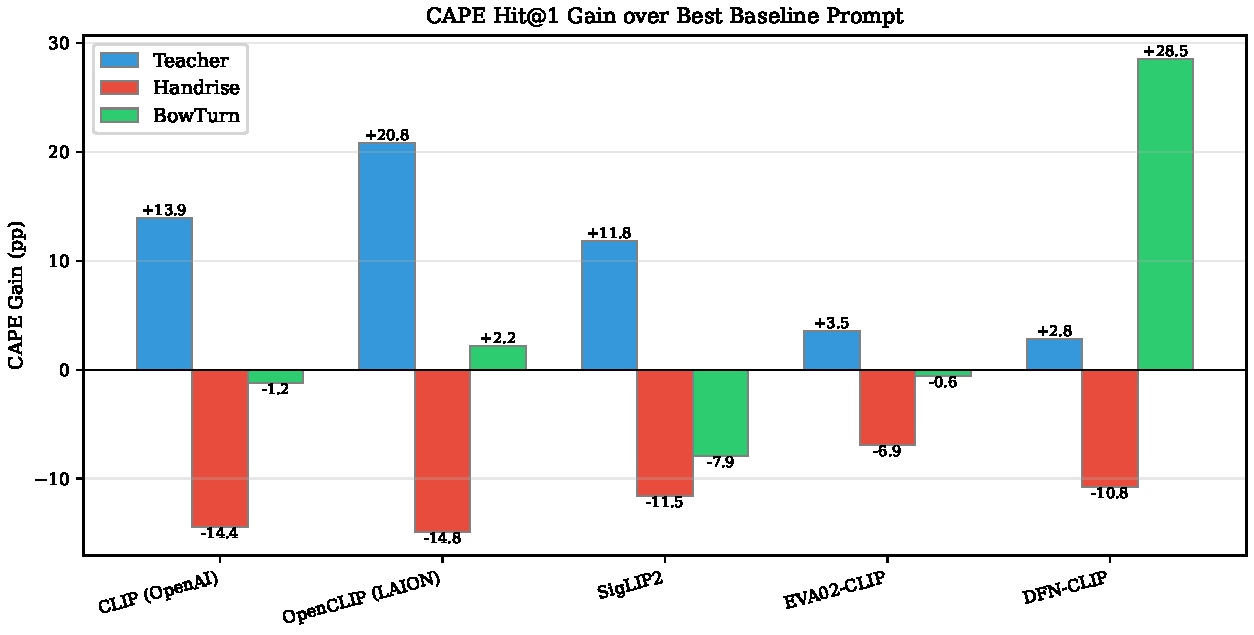
\includegraphics[width=0.85\textwidth]{fig_cape_gain.pdf}
\caption{CAPE Hit@1 gain (pp) over each model's best baseline prompt, by sub-dataset. Positive bars indicate CAPE improvement; negative bars indicate simpler prompts outperform CAPE. The consistent negative pattern on HandriseReadWrite supports task dependency.}
\label{fig:cape_gain}
\end{figure}

\subsubsection{E4: Robustness of CAPE Prompt Ensembles}
\label{sec:e4_robustness}

To assess whether CAPE's gains are robust to prompt wording rather than tied to a single handcrafted set, the prompt ensemble is perturbed along two axes: \emph{prompt count} (using one, two, or three prompts from Set~A), and \emph{wording} (replacing Set~A with independently written Set~B). A mixed-pool score is also reported by averaging over five random 3-prompt draws from the union of Set~A and Set~B.

Set~B follows the same three CAPE design principles (visual grounding, semantic diversity, and discriminative contrast) but uses independently written wording. The main benchmark fixes CAPE at $K=3$ prompts per class, whereas this section perturbs prompt count to probe sensitivity rather than to perform per-model tuning. The verbatim Set~A and Set~B prompts for all thirteen classes are released alongside the code (\texttt{scb5\_zeroshot/prompts/setAB\_examples.json}).

Robustness is strongly scene-dependent. TeacherBehavior is the least stable sub-dataset: all five models exhibit large Set~A vs. Set~B gaps and high mixed-prompt variance. SigLIP2 is the most extreme example, rising to 95.52\% with A(2) but dropping to 31.36\% with B(3). Because both values are reproduced in the archived robustness logs and JSON outputs, this swing is treated as an observed prompt-count and wording sensitivity effect rather than as a transcription artifact. In contrast, BowTurnHead is markedly more stable for several models, with mixed-prompt standard deviation as low as 1.94~pp for DFN-CLIP. HandriseReadWrite occupies a middle ground, where alternate wording often helps more than increasing prompt count.

The A(3) results should therefore be interpreted as robustness probes rather than duplicates of the fixed main setting. Small numerical differences from the main CAPE values arise because robustness uses an independently executed script. The full robustness matrix is provided in the release package to keep the main text concise.

\paragraph{Three-principle ablation.}
To attribute CAPE's gains to its design principles rather than to arbitrary prompt choices, each of the three CAPE design principles is individually degraded while keeping the other two and the prompt count ($K=3$) fixed: (\textsc{C1}) drop \emph{visual grounding} by replacing concrete physical descriptions with abstract conceptual phrasings; (\textsc{C2}) drop \emph{semantic diversity} by using three near-paraphrases of one viewpoint; (\textsc{C3}) drop \emph{discriminative contrast} by using generic per-class wording that does not separate classes (e.g., ``a classroom scene with a student'' for all student-action classes). \Cref{tab:cape_ablation} reports zero-shot results on TeacherBehavior (multi-label) and BowTurnHead (single-label) for the three backbones with cached features; HandriseReadWrite is summarized in the release package because the small label set leaves little room for principle separation.

On TeacherBehavior, dropping visual grounding causes the most consistent damage to Sample-F1 (CLIP/OpenAI $-17.6$~pp; SigLIP2 $-14.6$~pp) and almost completely collapses Hit@1 ($<10\%$ for all three backbones, indicating that abstract prompts no longer cluster by class identity). For DFN-CLIP, the visual-grounding ablation barely changes Sample-F1 (49.92 $\to$ 50.23) but still collapses Hit@1 from 45.90 to 5.68\%; this is consistent with DFN-CLIP's TeacherBehavior CAPE baseline being already weak ($45.86\%$ Hit@1, \Cref{tab:main_results})---i.e., DFN's text encoder is misaligned with the teacher-behavior label semantics for this prompt family rather than near a ceiling. Dropping discriminative contrast also reduces Sample-F1 substantially (CLIP $-16.7$~pp; SigLIP2 $-10.6$~pp) and collapses BowTurnHead single-label primary accuracy to the degenerate single-class floor of 36.63\% across all three backbones (the minority-class fraction reached when argmax ties drive every sample to a single fixed class), the cleanest signature of indistinguishable per-class prompts. In contrast, dropping only semantic diversity yields modest changes ($+2.3$ to $-4.2$~pp Sample-F1 on TeacherBehavior); for DFN-CLIP, both \textsc{C2} and \textsc{C3} ablations even \emph{slightly} raise the oracle Sample-F1 above CAPE-Full ($49.92 \to 51.05 / 54.94$). This is not a refutation of CAPE but a useful negative signal: when the backbone's text encoder is already misaligned with a label family on a given subset, adding more class-anchored prompt structure is not free---it can mildly hurt. CAPE should therefore be reported with per-backbone calibration rather than asserted as universally beneficial. Overall, the pattern indicates that CAPE's gains over a one-line baseline arise primarily from visual grounding and discriminative contrast, with semantic diversity acting as a secondary stabilizer.

\paragraph{Oracle vs.\ non-oracle multi-label F1.} Sample-F1, Macro-F1, and Micro-F1 in \Cref{tab:cape_ablation} use the standard CAPE-paper convention of predicting the top-$k$ classes per image where $k$ equals the ground-truth positive count for that image. This ``oracle-$k$'' convention informs the model how many labels to emit and is therefore an upper bound on what a fixed-threshold zero-shot system would achieve on the same logits. The headline LP-vs.-CAPE comparison in \Cref{tab:linear_probe_ml} uses the stricter non-oracle setting (CAPE multi-label F1 is taken from \Cref{tab:multilabel_eval}, which selects a fixed cosine threshold per backbone without oracle knowledge of $k$); under that protocol the LP advantage is even larger. Readers should therefore not directly compare \Cref{tab:cape_ablation} Sample-F1 numbers to \Cref{tab:linear_probe_ml} Sample-F1 numbers, and should treat the former as relative ablation deltas rather than as absolute deployable F1.

\begin{table}[H]
\caption{CAPE three-principle ablation. \textsc{C0} is the original CAPE-A. Each ablation degrades one principle while holding the other two and prompt count ($K=3$) constant. Multi-label F1 metrics are reported on TeacherBehavior; Hit@1 on BowTurnHead is the single-label primary accuracy (505 images, 2 classes; single-label majority floor $63.37\%$, multi-label Hit@1 majority floor $90.69\%$). Italic numbers indicate the degenerate single-class floor (here $36.63\%$, the minority-class fraction reached when the discriminative-contrast ablation collapses argmax to a single fixed class). Cached image features are reused; only text features are recomputed. Bold marks each row's strongest CAPE-Full vs.\ ablation contrast.}
\label{tab:cape_ablation}
\centering
\small
\begin{tabular}{l l cccc c}
\toprule
& & \multicolumn{4}{c}{\textbf{TeacherBehavior}} & \textbf{BowTurnHead} \\
\cmidrule(lr){3-6}\cmidrule(lr){7-7}
\textbf{Backbone} & \textbf{Condition} & Hit@1 & Sample-F1 & Macro-F1 & Micro-F1 & Hit@1 \\
\midrule
\multirow{4}{*}{CLIP (OpenAI)}
 & \textsc{C0} CAPE-Full        & 84.32 & \textbf{66.57} & 54.19 & 69.63 & \textbf{63.56} \\
 & \textsc{C1} $\neg$VisGround  &  7.59 & 48.94 & 40.95 & 53.66 & 44.16 \\
 & \textsc{C2} $\neg$SemDiv     & 85.80 & 68.89 & 54.79 & 72.23 & 45.94 \\
 & \textsc{C3} $\neg$Discrim    & 56.82 & 49.85 & 48.06 & 54.63 & \textit{36.63} \\
\midrule
\multirow{4}{*}{SigLIP2}
 & \textsc{C0} CAPE-Full        & 85.49 & \textbf{64.97} & 56.67 & 68.55 & \textbf{64.75} \\
 & \textsc{C1} $\neg$VisGround  &  7.13 & 50.39 & 42.57 & 55.58 & 40.20 \\
 & \textsc{C2} $\neg$SemDiv     & 79.38 & 60.76 & 56.11 & 64.33 & 56.24 \\
 & \textsc{C3} $\neg$Discrim    & 68.64 & 54.32 & 51.42 & 58.57 & \textit{36.63} \\
\midrule
\multirow{4}{*}{DFN-CLIP}
 & \textsc{C0} CAPE-Full        & 45.90 & 49.92 & 52.72 & 56.26 & \textbf{68.32} \\
 & \textsc{C1} $\neg$VisGround  &  5.68 & 50.23 & 38.97 & 54.53 & 40.20 \\
 & \textsc{C2} $\neg$SemDiv     & 37.62 & 51.05 & 48.39 & 56.17 & 41.78 \\
 & \textsc{C3} $\neg$Discrim    & 68.02 & 54.94 & 51.52 & 59.44 & \textit{36.63} \\
\bottomrule
\end{tabular}
\end{table}

\subsubsection{E5: Descriptive Cross-Model Summary}
\label{sec:e5}

To provide a compact descriptive summary, each model's best Hit@1 (across all prompts) per sub-dataset is averaged across the three non-degenerate sub-datasets (\Cref{tab:model_ranking}). This summary should not be interpreted as a formal global ranking, because the three subsets differ in label structure and difficulty and because the best prompt is selected post hoc for each model.
Under this descriptive average, CLIP (OpenAI) and SigLIP2 occupy the highest summary values, whereas OpenCLIP (LAION), EVA02-CLIP, and DFN-CLIP show stronger subset dependence.
The table is therefore used only to summarize cross-subset dispersion, not to claim a universally best backbone for classroom activity recognition.

\begin{table}[H]
\caption{Descriptive summary of average best Hit@1 (\%) across three sub-datasets. Because the best prompt is selected separately for each model and the subsets are heterogeneous, these averages are reported for compact comparison only, not as a formal statistical ranking. Selected best-prompt strategies are CLIP (OpenAI): Teacher=CAPE, Handrise=detailed, BowTurn=detailed; SigLIP2: Teacher=CAPE, Handrise=detailed, BowTurn=simple; OpenCLIP (LAION): Teacher=CAPE, Handrise=action, BowTurn=CAPE; EVA02-CLIP: Teacher=action, Handrise=label-only, BowTurn=CAPE; DFN-CLIP: Teacher=CAPE, Handrise=label-only, BowTurn=CAPE.}
\label{tab:model_ranking}
\centering
\begin{tabular}{lcccr}
\toprule
\textbf{Model} & \textbf{Teacher} & \textbf{Handrise} & \textbf{BowTurn} & \textbf{Avg.} \\
\midrule
CLIP (OpenAI) & 84.14 & 82.41 & 90.69 & \textbf{85.75} \\
SigLIP2 & \textbf{85.56} & 76.00 & 90.30 & 83.95 \\
OpenCLIP (LAION) & 54.94 & \textbf{84.56} & 92.87 & 77.46 \\
EVA02-CLIP & 78.86 & 82.23 & 65.35 & 75.48 \\
DFN-CLIP & 45.86 & 84.50 & \textbf{93.27} & 74.54 \\
\bottomrule
\end{tabular}
\end{table}

\subsection{Reliability and supervised baselines}

\subsubsection{E6: Error Analysis and Class-Level Behavior}
\label{sec:e6}

To move beyond aggregate Hit@1, per-class prediction patterns are analyzed using confusion matrices (\Cref{fig:cm_teacher}) and per-class recall (\Cref{fig:per_class}).

\begin{figure}[H]
\centering
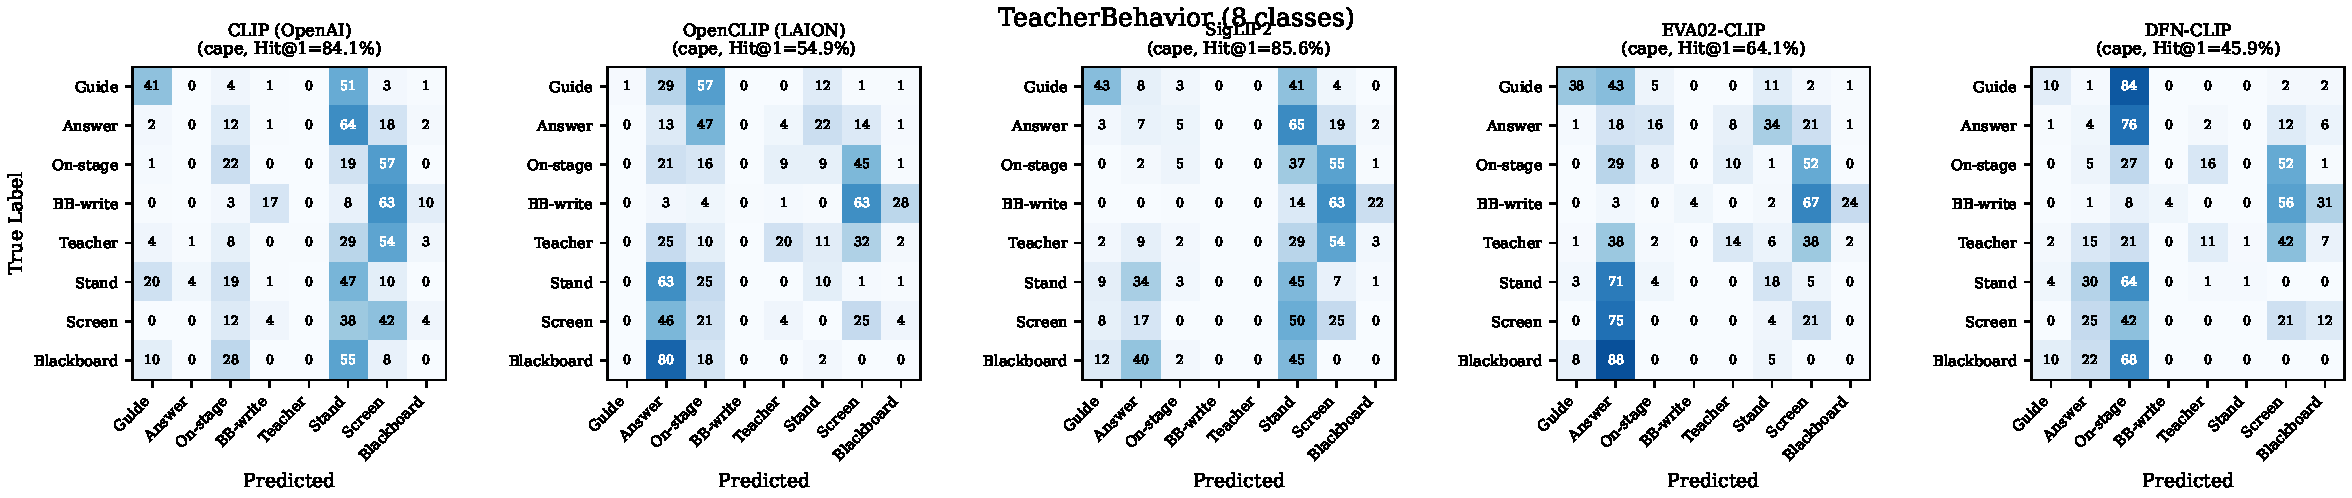
\includegraphics[width=\textwidth]{fig_confusion_matrix_teacher.pdf}
\caption{Normalized confusion matrices (row = true, column = predicted, values in \%) for TeacherBehavior under each model's best prompt. All five models heavily over-predict ``teacher'' and ``stand,'' which together account for $>$90\% of predictions.}
\label{fig:cm_teacher}
\end{figure}

The confusion matrices reveal a consistent failure mode: all five models collapse predictions toward the ``teacher'' and ``stand'' classes, which have the highest base rates (45.0\% and 5.2\% of labels, respectively, but appear in $>$97\% of images as co-occurring labels).
Minority classes such as ``screen'' (0.7\%) and ``blackboard'' (1.2\%) are almost never predicted, explaining the $<$14.5\% macro~F1 despite $>$84\% Hit@1.

\begin{figure}[H]
\centering
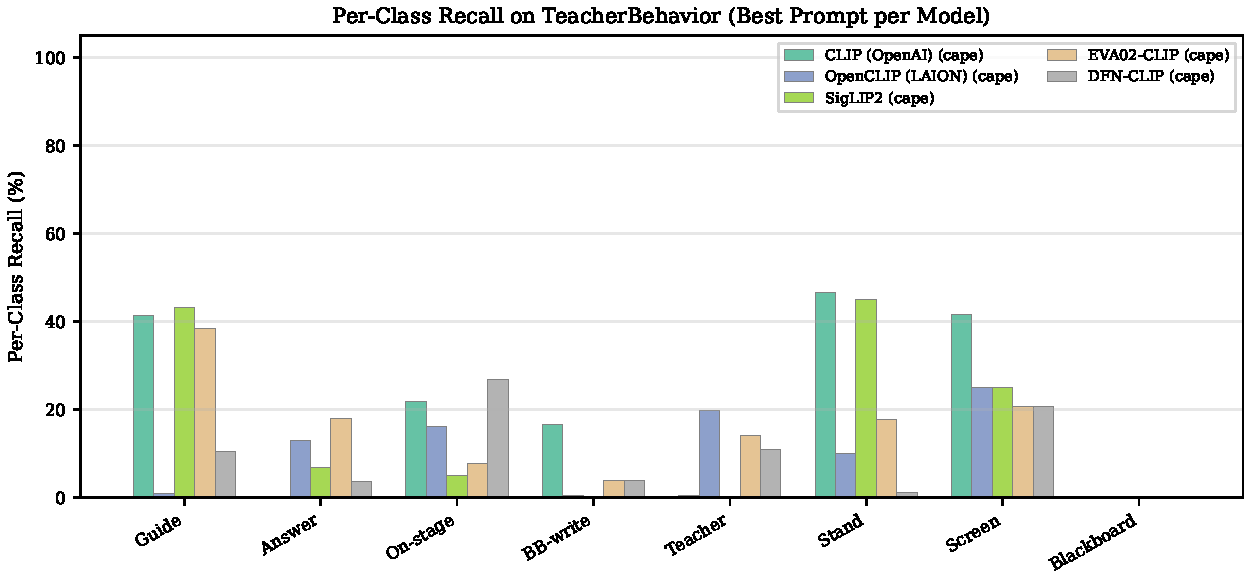
\includegraphics[width=\textwidth]{fig_per_class_teacher.pdf}
\caption{Per-class recall (\%) on TeacherBehavior for each model (best prompt). ``Teacher'' and ``stand'' achieve high recall; ``screen'' and ``blackboard'' are near zero.}
\label{fig:per_class}
\end{figure}

\Cref{fig:per_class} quantifies this imbalance: ``teacher'' recall exceeds 60\% for four of five models under their best prompt, while ``screen'' recall is 0\% for all models except SigLIP2 (which achieves $\sim$4\% via detailed prompts).
This is not a model failure \textit{per se}, but a consequence of multi-label structure: a model predicting ``teacher'' is correct for 45\% of images, while predicting ``screen'' is correct for only 0.7\%.
Zero-shot models follow the path of least resistance in the shared embedding space.

\Cref{fig:pred_dist} further illustrates the prediction distribution mismatch.

\begin{figure}[H]
\centering
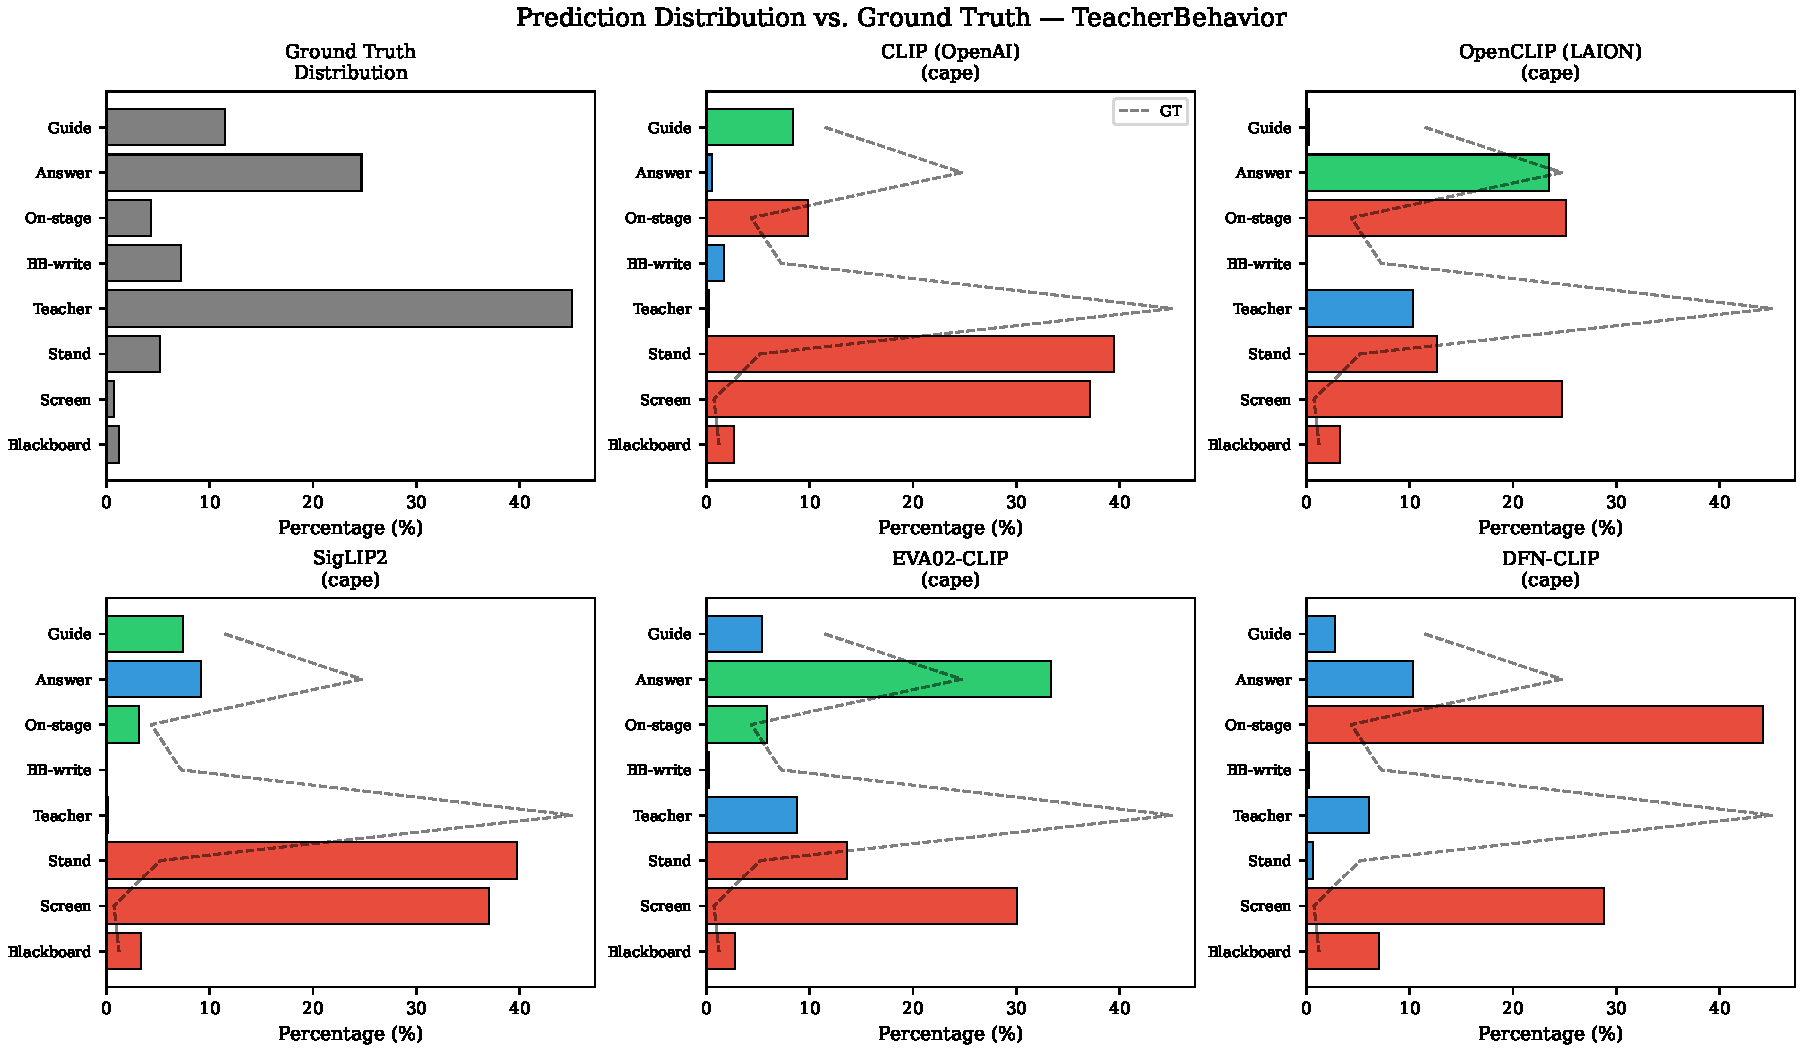
\includegraphics[width=\textwidth]{fig_prediction_distribution.pdf}
\caption{Prediction distribution (colored bars) vs.\ ground-truth distribution (dashed line) for TeacherBehavior. Red indicates over-prediction; blue indicates under-prediction relative to the true distribution.}
\label{fig:pred_dist}
\end{figure}

The heatmap in \Cref{fig:heatmap} provides a compact overview of the full 5~model $\times$ 5~prompt interaction across all three sub-datasets.

\begin{figure}[H]
\centering
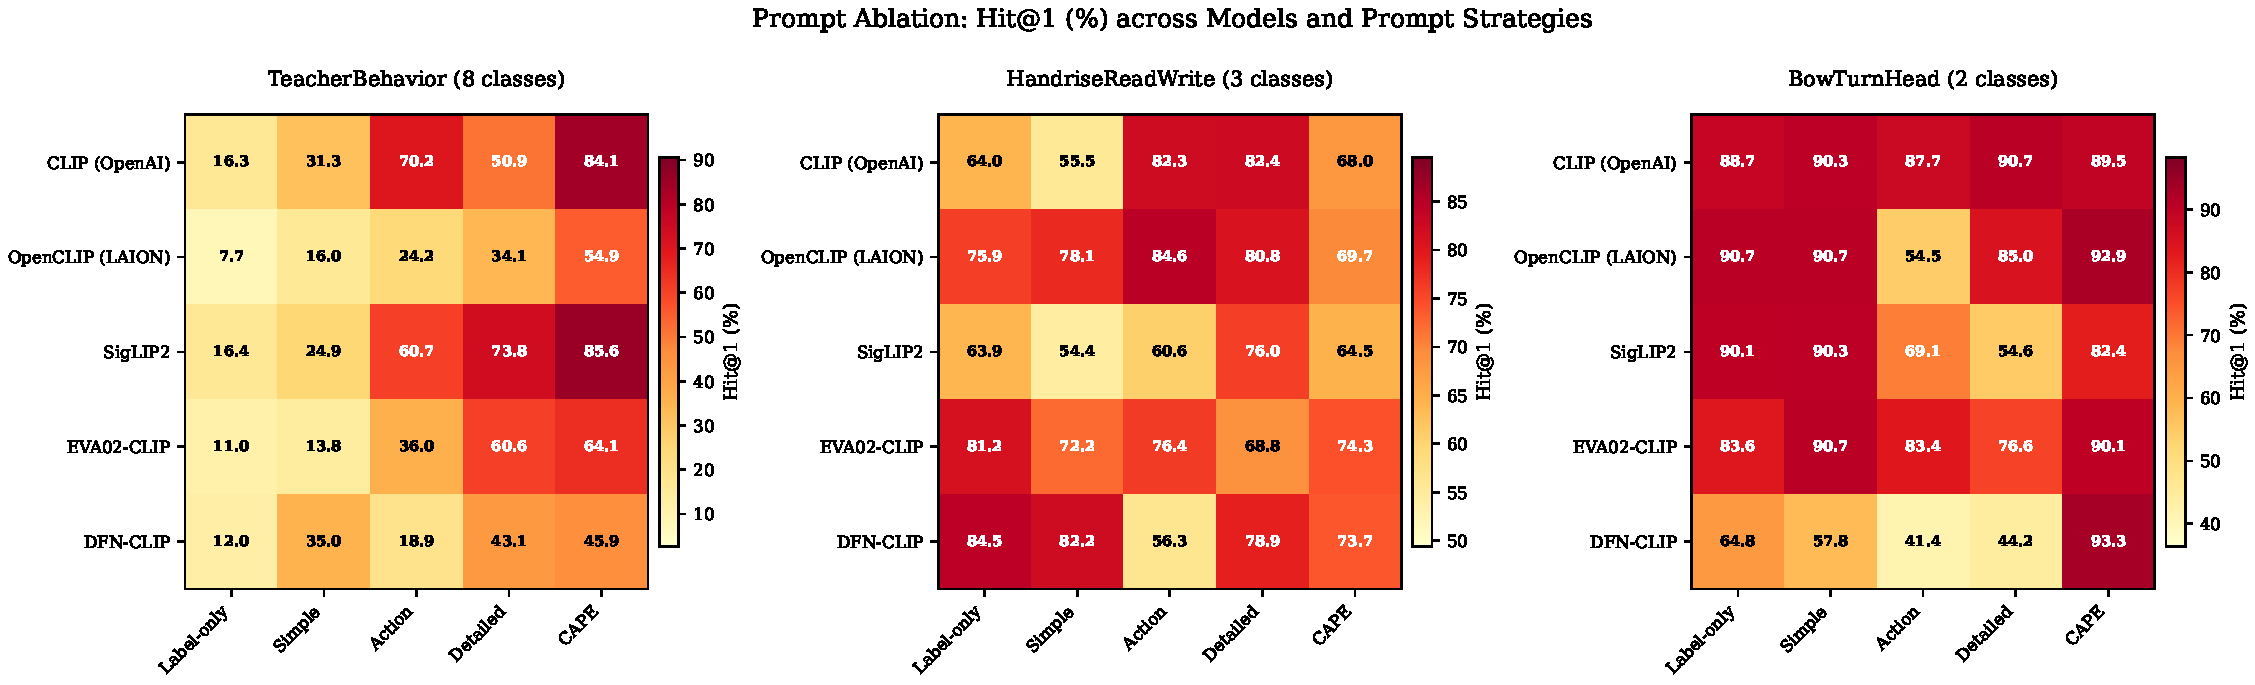
\includegraphics[width=\textwidth]{fig_prompt_ablation_heatmap.pdf}
\caption{Hit@1 (\%) heatmap across five models and five prompt strategies for each sub-dataset. The strong column effect (prompt strategy) on TeacherBehavior and the strong row effect (model choice) on HandriseReadWrite are clearly visible.}
\label{fig:heatmap}
\end{figure}

Two patterns emerge from the heatmap:
(1)~On TeacherBehavior, the dominant gradient runs left-to-right (prompt complexity), confirming that prompt design is the primary factor.
(2)~On HandriseReadWrite, the pattern is more model-dependent, with LAION and DFN achieving high scores across multiple prompt strategies while SigLIP2 is more prompt-sensitive.
This corroborates the task-dependent nature of both prompt and model selection.


\subsubsection{E7: Supervised Baseline via Linear Probing}
\label{sec:e7_linear_probe}

To contextualize zero-shot performance, a supervised baseline is established by training a logistic regression classifier on frozen CLIP image features. For each backbone, image features are extracted with the frozen ViT-Large vision encoder \emph{without} L2-renormalisation across train/val (the encoder's output convention is preserved as released), then standardised with a per-feature \texttt{StandardScaler} fitted on the training split only and applied to validation. A multinomial logistic regression is fitted on this standardised representation with L2 regularisation (\texttt{scikit-learn} default \texttt{LogisticRegression(C=1.0, max\_iter=1000, solver="lbfgs")}, no class re-weighting, no validation-set hyperparameter search) on the official training split provided by the dataset release ($N=8984$ images for TeacherBehavior, $\approx$3500 for HandriseReadWrite, $\approx$2050 for BowTurnHead). For HandriseReadWrite and BowTurnHead, this single multinomial model yields a per-image class index, and accuracy is reported on the validation split. For TeacherBehavior, an additional set of \emph{per-class binary classifiers} (one-vs-rest \texttt{LogisticRegression} with the same hyperparameters) is trained for multi-label evaluation; binary predictions use the default decision boundary $p\geq0.5$, and Sample-F1, Macro-F1, and Micro-F1 are reported in \Cref{tab:linear_probe_ml} without per-class threshold tuning on the validation split. No image augmentation, no feature fine-tuning, and no validation-set early stopping is used---the comparison isolates the value of labeled data alone and makes the LP numbers directly reproducible from the released cached features.

\Cref{tab:linear_probe} presents the results. Two findings are observed. First, on single-label metrics, the supervised advantage is clear: on HandriseReadWrite, linear probing reaches 83.18\% accuracy (CLIP) versus 67.98\% for CAPE---a +15.2~pp supervised advantage. On BowTurnHead, models are roughly comparable.

Second, the TeacherBehavior comparison requires nuance given the multi-label structure of the dataset and the potential for metric artifacts. The linear probe trained on primary labels achieves 71--77\% Hit@1 versus 46--86\% for zero-shot CAPE. However, when evaluated with proper multi-label metrics using per-class binary classifiers, the linear probe achieves Sample-F1 of 88--90\%, Macro-F1 of 68--78\%, and Micro-F1 of 89--91\% (\Cref{tab:linear_probe_ml}), substantially outperforming zero-shot CAPE (Sample-F1 60--66\%, Macro-F1 49--61\%, Micro-F1 61--70\% from \Cref{tab:multilabel_eval}). These results indicate that \textbf{the zero-shot advantage on Hit@1 is largely an artifact of lenient multi-label evaluation}, not a genuine superiority over supervised learning. Under the same multi-label protocol, supervised linear probing with 8984 labeled training images remains stronger across all five backbones.

\begin{table}[H]
\caption{Linear probe (LP) vs.\ zero-shot CAPE: single-label comparison. LP trains a logistic regression on frozen ViT-L features using primary labels. Hit@1 uses multi-label evaluation; Acc and Macro-F1 use primary-label assignment. Best per dataset in bold.}
\label{tab:linear_probe}
\centering
\small
\setlength{\tabcolsep}{3pt}
\begin{tabular}{l cc cc cc}
\toprule
 & \multicolumn{2}{c}{\textbf{TeacherBehavior}} & \multicolumn{2}{c}{\textbf{HandriseReadWrite}} & \multicolumn{2}{c}{\textbf{BowTurnHead}} \\
\cmidrule(lr){2-3}\cmidrule(lr){4-5}\cmidrule(lr){6-7}
\textbf{Model backbone} & LP Hit@1 & ZS Hit@1 & LP Acc & ZS Hit@1 & LP Acc & ZS Hit@1 \\
\midrule
CLIP (OpenAI) & 77.10 & \textbf{84.14} & \textbf{83.18} & 67.98 & 63.96 & \textbf{89.50} \\
OpenCLIP (LAION) & 76.85 & 54.94 & \textbf{80.49} & 69.72 & 66.73 & \textbf{92.87} \\
SigLIP2 & 76.33 & \textbf{85.56} & \textbf{73.19} & 64.45 & 67.33 & \textbf{82.38} \\
EVA02-CLIP & 75.77 & 64.35 & \textbf{76.78} & 60.62 & 59.21 & \textbf{65.35} \\
DFN-CLIP & 71.98 & 45.86 & \textbf{80.61} & 73.73 & 60.20 & \textbf{93.27} \\
\bottomrule
\end{tabular}
\end{table}

\begin{table}[H]
\caption{Multi-label comparison on TeacherBehavior: supervised LP (per-class binary classifiers trained on 8984 images) vs.\ zero-shot CAPE (from \Cref{tab:multilabel_eval}). LP achieves substantially higher multi-label F1 across all backbones, confirming that the zero-shot Hit@1 advantage in \Cref{tab:linear_probe} is an artifact of the lenient evaluation.}
\label{tab:linear_probe_ml}
\centering
\small
\setlength{\tabcolsep}{3.5pt}
\begin{tabular}{l cccc cccc}
\toprule
 & \multicolumn{4}{c}{\textbf{Supervised LP (multi-label)}} & \multicolumn{4}{c}{\textbf{Zero-Shot CAPE (multi-label)}} \\
\cmidrule(lr){2-5}\cmidrule(lr){6-9}
\textbf{Backbone} & Hit@1 & S-F1 & Ma-F1 & Mi-F1 & Hit@1 & S-F1 & Ma-F1 & Mi-F1 \\
\midrule
CLIP & \textbf{77.10} & 88.61 & \textbf{78.42} & 90.64 & 84.14 & 64.19 & 55.62 & 66.38 \\
LAION & 76.85 & 88.83 & 75.74 & 90.55 & 54.94 & 65.20 & 57.04 & 67.38 \\
SigLIP2 & 76.33 & 87.53 & 68.02 & 89.50 & \textbf{85.56} & 59.94 & 49.03 & 61.19 \\
EVA02 & 75.77 & \textbf{89.62} & 77.31 & \textbf{91.02} & 64.35 & \textbf{66.46} & \textbf{60.50} & \textbf{69.99} \\
DFN & 71.98 & 88.52 & 73.60 & 90.42 & 45.86 & 63.59 & 57.07 & 66.16 \\
\bottomrule
\end{tabular}
\\[3pt]
{\footnotesize S-F1 = Sample-F1, Ma-F1 = Macro-F1, Mi-F1 = Micro-F1. Bold marks the best backbone per metric column. LP outperforms zero-shot CAPE on every F1 metric for every backbone, while zero-shot Hit@1 occasionally exceeds LP Hit@1 because Hit@1 uses the lenient multi-label criterion ($\hat{y}\in G$) whereas LP is trained against primary labels.}
\end{table}


\subsubsection{E8: Bootstrap Confidence Intervals}
\label{sec:e8_bootstrap}

To quantify statistical reliability on small datasets, 95\% bootstrap confidence intervals (1000 resamples with replacement) are computed for the CAPE zero-shot Hit@1 setting on all sub-datasets. \Cref{tab:bootstrap_ci} reports the intervals. These intervals quantify uncertainty for the CAPE configuration only; they are not formal significance tests for the post hoc best-prompt averages in \Cref{tab:model_ranking}.

On BowTurnHead (505 images), the bootstrap intervals are reported on the stricter \emph{single-label primary accuracy} (the majority floor of which is 63.37\%), and the 95\% CI widths range from 7 to 9~pp with substantial overlap between models. For example, CLIP achieves 63.4\% [59.4, 67.3] while DFN-CLIP achieves 68.3\% [64.6, 72.1]---the intervals overlap, indicating \textbf{no statistically significant difference} at the 95\% level. The corresponding multi-label Hit@1 figures in \Cref{tab:main_results} (89.50\% / 93.27\%) sit just $\sim$0--3~pp above the multi-label majority floor of 90.69\%; \textbf{the headline ranking on this subset should therefore be read as a small effect on top of a near-saturated lenient metric}, not as a strong cross-model gap. Similarly, on TeacherBehavior, SigLIP2 (85.5\% [84.4, 86.7]) and CLIP (84.1\% [83.0, 85.4]) show overlapping CIs despite a nominal 1.4~pp gap.

On HandriseReadWrite, CIs are narrower ($\sim$5~pp width) due to the larger sample size, and model differences are somewhat more reliable, though all CAPE Hit@1 values cluster between 56--61\%.

\paragraph{Paired-bootstrap significance test.} Marginal CIs are conservative for cross-model comparison because the same images are scored by every backbone. \Cref{tab:paired_bootstrap} therefore reports a \emph{paired} bootstrap (5000 resamples with replacement, two-sided, seed 42) on the per-sample CAPE Hit@1 indicators, computed directly from the released CAPE logits caches (\texttt{data/feature\_cache/}) for the three backbones with full-coverage caches (CLIP/OpenAI, DFN-CLIP, SigLIP2). Three observations follow. (i) On TeacherBehavior, OpenAI vs.\ SigLIP2 is \emph{not} significant ($p=0.089$), confirming the visual CI overlap; both are clearly different from DFN-CLIP ($p<10^{-3}$). (ii) On BowTurnHead, OpenAI vs.\ DFN is paired-significant ($\Delta=-4.75$~pp, 95\% CI $[-7.5,-2.2]$, $p<10^{-3}$) even though the marginal CIs in \Cref{tab:bootstrap_ci} overlap, illustrating that overlapping marginal CIs do not imply paired non-significance. (iii) On HandriseReadWrite, OpenAI vs.\ SigLIP2 is significant ($p=0.006$) but the effect size is small ($\Delta=1.7$~pp). These results refine the conservative ranking statements made elsewhere in the paper without changing any qualitative conclusion.

\begin{table}[H]
\caption{Paired-bootstrap significance test for CAPE per-sample Hit@1, computed on the cached \texttt{logits\_cape} fields. ``Acc'' columns are point estimates from the same caches (multi-label argmax for TeacherBehavior; single-label primary accuracy for HandriseReadWrite/BowTurnHead, identical in definition to \Cref{tab:bootstrap_ci}). $\Delta=\text{Acc}_A-\text{Acc}_B$ in pp; 95\% CI is from 5000 paired bootstrap resamples; $p$ is two-sided. Pairs are restricted to backbones with full-coverage feature caches.}
\label{tab:paired_bootstrap}
\centering
\small
\setlength{\tabcolsep}{4pt}
\begin{tabular}{l ll cc r r l}
\toprule
\textbf{Subset} & \textbf{A} & \textbf{B} & $\text{Acc}_A$ & $\text{Acc}_B$ & $\Delta$ (pp) & 95\% CI (pp) & $p$ \\
\midrule
Teacher  & OpenAI  & DFN     & 84.32 & 45.90 & $+38.43$ & $[+36.6,+40.3]$ & $<10^{-3}$ \\
Teacher  & OpenAI  & SigLIP2 & 84.32 & 85.49 & $-1.17$  & $[-2.5,+0.2]$    & $0.089$    \\
Teacher  & DFN     & SigLIP2 & 45.90 & 85.49 & $-39.60$ & $[-41.4,-38.0]$ & $<10^{-3}$ \\
\midrule
Handrise & OpenAI  & DFN     & 57.99 & 56.91 & $+1.08$  & $[-0.1,+2.3]$    & $0.089$    \\
Handrise & OpenAI  & SigLIP2 & 57.99 & 56.25 & $+1.74$  & $[+0.5,+3.0]$    & $0.006$    \\
Handrise & DFN     & SigLIP2 & 56.91 & 56.25 & $+0.66$  & $[-0.5,+1.9]$    & $0.306$    \\
\midrule
BowTurn  & OpenAI  & DFN     & 63.56 & 68.32 & $-4.75$  & $[-7.5,-2.2]$    & $<10^{-3}$ \\
BowTurn  & OpenAI  & SigLIP2 & 63.56 & 64.75 & $-1.19$  & $[-5.7,+3.4]$    & $0.635$    \\
BowTurn  & DFN     & SigLIP2 & 68.32 & 64.75 & $+3.56$  & $[-0.6,+7.7]$    & $0.104$    \\
\bottomrule
\end{tabular}
\end{table}

\begin{table}[H]
\caption{Bootstrap 95\% confidence intervals for CAPE zero-shot top-1 performance (\%). Mean [lower, upper] from 1000 bootstrap resamples. \textbf{Metric note:} On TeacherBehavior the value is multi-label Hit@1 ($\hat{y}_i\in G_i$, identical in definition to \Cref{tab:main_results}); on HandriseReadWrite and BowTurnHead the value is single-label primary accuracy ($\hat{y}_i=y^{\text{primary}}_i$), which is stricter than the multi-label Hit@1 reported in \Cref{tab:main_results}. As a reference, the multi-label majority floor on BowTurnHead is 90.69\% (any prediction landing on the larger label set ``turn-head'' counts as a hit); the corresponding single-label primary-accuracy majority floor is 63.37\%.}
\label{tab:bootstrap_ci}
\centering
\small
\setlength{\tabcolsep}{3pt}
\begin{tabular}{l ccc}
\toprule
\textbf{Model} & \textbf{TeacherBehavior} & \textbf{HandriseReadWrite} & \textbf{BowTurnHead} \\
\midrule
CLIP (OpenAI) & 84.1 [83.0, 85.4] & 58.0 [55.7, 60.4] & 63.4 [59.4, 67.3] \\
OpenCLIP (LAION) & 55.0 [53.4, 56.8] & 60.9 [58.5, 63.1] & 67.7 [63.8, 71.5] \\
SigLIP2 & 85.5 [84.4, 86.7] & 56.3 [53.9, 58.7] & 64.7 [60.6, 68.9] \\
EVA02-CLIP & 64.4 [62.8, 66.1] & 60.7 [58.3, 63.0] & 65.3 [61.2, 69.3] \\
DFN-CLIP & 45.9 [44.2, 47.5] & 57.0 [54.6, 59.3] & 68.3 [64.6, 72.1] \\
\bottomrule
\end{tabular}
\end{table}


\subsection{Independent validation and extensions}

\subsubsection{E9: Independent Prompt Validation (Blind Set~C)}
\label{sec:e9_blind}

A potential concern with CAPE is unconscious overfitting: the same authors design and evaluate prompts on the same test set. To assess this, a \emph{blind} prompt set (Set~C) is constructed, written solely from class names without examining any dataset images. Set~C simulates what a third party---or a language model---would produce given only the category labels and no domain knowledge of Chinese classroom footage.

\Cref{tab:blind_prompts} compares Hit@1 across three prompt sets: Set~A (original CAPE), Set~B (alternate wording by the same authors), and Set~C (blind).

\begin{table}[H]
\caption{Hit@1 and Macro-F1 (\%) comparison of CAPE Set~A (original), Set~B (alternate wording), and Set~C (blind, written without viewing dataset images). Macro-F1 uses primary-label assignment for TeacherBehavior and standard single-label assignment for the other two sub-datasets.}
\label{tab:blind_prompts}
\centering
\small
\setlength{\tabcolsep}{2.5pt}
\begin{tabular}{l cc@{~~}c cc@{~~}c cc@{~~}c}
\toprule
 & \multicolumn{3}{c}{\textbf{TeacherBehavior}} & \multicolumn{3}{c}{\textbf{HandriseReadWrite}} & \multicolumn{3}{c}{\textbf{BowTurnHead}} \\
\cmidrule(lr){2-4}\cmidrule(lr){5-7}\cmidrule(lr){8-10}
\textbf{Model} & A & B & C & A & B & C & A & B & C \\
\midrule
\multicolumn{10}{l}{\textit{Hit@1}} \\
CLIP & 84.1 & 72.9 & 91.9 & 58.0 & 70.6 & 36.8 & 63.4 & 54.3 & 38.0 \\
LAION & 55.0 & 35.4 & 92.2 & 60.8 & 63.6 & 61.0 & 67.7 & 61.2 & 53.1 \\
SigLIP2 & 85.5 & 31.4 & 91.7 & 56.3 & 70.2 & 65.1 & 64.7 & 48.3 & 67.1 \\
EVA02 & 64.4 & 39.2 & 92.1 & 60.6 & 71.2 & 56.9 & 65.3 & 53.7 & 53.7 \\
DFN & 45.9 & 22.2 & 92.4 & 56.9 & 72.4 & 46.3 & 68.3 & 62.2 & 58.2 \\
\addlinespace
\multicolumn{10}{l}{\textit{Macro-F1}} \\
CLIP & 12.7 & 10.9 & 10.4 & 38.8 & 53.0 & 32.8 & 43.4 & 50.0 & 29.7 \\
LAION & 7.5 & 12.8 & 10.3 & 42.1 & 45.2 & 51.3 & 51.2 & 60.2 & 53.1 \\
SigLIP2 & 10.0 & 10.6 & 11.9 & 34.8 & 51.9 & 54.2 & 59.8 & 48.2 & 51.8 \\
EVA02 & 14.4 & 13.6 & 10.9 & 43.7 & 51.0 & 47.3 & 47.9 & 53.6 & 53.5 \\
DFN & 7.1 & 10.8 & 12.3 & 38.2 & 52.2 & 37.7 & 53.5 & 60.4 & 54.7 \\
\bottomrule
\end{tabular}
\end{table}

The results indicate a methodological issue. On TeacherBehavior, Set~C achieves $\sim$92\% Hit@1 across all models---far above Set~A (45--86\%). However, this apparent superiority is an \emph{artifact of multi-label evaluation}. Set~C's generic prompts (e.g., ``a person in the role of a teacher or instructor'' for class ``teacher'') systematically predict the two most prevalent labels (``teacher'' at 92.6\% and ``stand'' at 97.2\%), which appear in nearly every image. Because Hit@1 succeeds when the prediction matches \emph{any} ground-truth label, Set~C achieves high Hit@1 by exploiting label co-occurrence rather than discriminating between classes. This is confirmed by the Macro-F1 scores: Set~C achieves only 10--12\% Macro-F1 on TeacherBehavior, comparable to or below Set~A's values, demonstrating limited ability to distinguish minority classes.

Conversely, on HandriseReadWrite and BowTurnHead---where multi-label inflation is absent---Set~C is usually weaker than the domain-aware prompts and does not show a stable advantage across models or metrics, confirming that \textbf{domain-aware prompt design (CAPE) provides genuine value for fine-grained activity discrimination}. The blind set lacks the visual grounding and discriminative contrast that CAPE's design principles provide.

This analysis also serves as a cautionary note: \textbf{Hit@1 alone is insufficient for evaluating prompts on multi-label data.} Future work should pair Hit@1 with class-discriminative metrics (Macro-F1, per-class recall) to avoid rewarding degenerate predictions that exploit label co-occurrence.


\subsubsection{E10: Multi-Label Evaluation}
\label{sec:e10_multilabel}

Because primary-label evaluation is lenient on multi-label data, proper multi-label metrics on TeacherBehavior are computed using two approaches: (1)~thresholding cosine similarity scores at various cutoffs to produce multi-label predictions, and (2)~using top-$k$ predictions as surrogate multi-label outputs. \Cref{tab:multilabel_eval} reports the best configuration per model.

\begin{table}[H]
\caption{Multi-label evaluation on TeacherBehavior (CAPE zero-shot). Best threshold or top-$k$ per model selected by Sample-F1.}
\label{tab:multilabel_eval}
\centering
\small
\begin{tabular}{llccc}
\toprule
\textbf{Model} & \textbf{Strategy} & \textbf{Sample-F1} & \textbf{Macro-F1} & \textbf{Micro-F1} \\
\midrule
CLIP (OpenAI) & $\tau=0.20$ & 64.19 & 55.62 & 66.38 \\
OpenCLIP (LAION) & $\tau=0.20$ & 65.20 & 57.04 & 67.38 \\
SigLIP2 & top-3 & 59.94 & 49.03 & 61.19 \\
EVA02-CLIP & $\tau=0.20$ & \textbf{66.46} & \textbf{60.50} & \textbf{69.99} \\
DFN-CLIP & $\tau=0.15$ & 63.59 & 57.07 & 66.16 \\
\bottomrule
\end{tabular}
\end{table}

At the optimal threshold ($\tau=0.20$), most models achieve Sample-F1 of 64--66\% and Macro-F1 of 55--60\%. EVA02-CLIP achieves the highest multi-label Macro-F1 (60.50\%) despite ranking only third in Hit@1 (64.35\%)---an inversion that highlights the complementary nature of the two metrics. SigLIP2, which tops the Hit@1 ranking (85.56\%), achieves only 49.03\% multi-label Macro-F1, revealing that its high Hit@1 is partly driven by predicting high-prevalence labels rather than by genuinely discriminating across all eight categories.

These multi-label metrics provide a more faithful picture of zero-shot model capabilities on inherently multi-label educational data and complement Hit@1 in benchmarking studies.


\subsubsection{E11: Cross-Family and Cross-Prompt Validation}
\label{sec:e11_ex}

Two cross-family analyses examine the generality of the main conclusions beyond CLIP-family encoders: (1) a comparison against contemporary MLLMs on the same three SCB5 subsets, and (2) a direct comparison between EVA02-CLIP under CAPE and EVA02-CLIP under its best prompt strategy after checking all five prompt options. The MLLM comparison uses three Ollama-distributed models, \texttt{qwen3.5:9b}, \texttt{qwen3.5:27b}, and \texttt{gemma4:26b}, in a zero-shot setting and reports both Hit@1 and Macro-F1 under the deterministic protocol defined in \Cref{sec:mllm_protocol}.\footnote{The names \texttt{qwen3.5:Xb} and \texttt{gemma4:Yb} refer to local Ollama-distribution tags actually deployed in this study; they are not identical to upstream Hugging Face release names of the Qwen and Gemma series, and exact tag identifiers and quantization are recorded in the release package for reproducibility.}

\begin{table}[H]
\caption{Cross-family validation: MLLM comparison against the best zero-shot CLIP reference. ``Best CLIP reference'' denotes the strongest CLIP-family configuration on each subset (TeacherBehavior: SigLIP2+CAPE; HandriseReadWrite: OpenCLIP+action; BowTurnHead: DFN-CLIP+CAPE). Values are percentages. Weighted metrics are sample-size-weighted over the three subsets ($N=5416$). \textit{Protocol caveat:} on TeacherBehavior, MLLMs are constrained to emit a single label, whereas CLIP-family models expose a full similarity vector; the cross-family comparison should therefore be read as a single-choice proxy under a shared scorer (\Cref{sec:mllm_protocol}), not as an exact mechanistic match.}
\label{tab:mllm_validation}
\centering
\small
\setlength{\tabcolsep}{3pt}
\begin{tabular}{l cc cc cc cc}
\toprule
 & \multicolumn{2}{c}{\textbf{TeacherBehavior}} & \multicolumn{2}{c}{\textbf{HandriseReadWrite}} & \multicolumn{2}{c}{\textbf{BowTurnHead}} & \multicolumn{2}{c}{\textbf{Weighted}} \\
\cmidrule(lr){2-3}\cmidrule(lr){4-5}\cmidrule(lr){6-7}\cmidrule(lr){8-9}
\textbf{Model} & Hit@1 & Macro-F1 & Hit@1 & Macro-F1 & Hit@1 & Macro-F1 & Hit@1 & Macro-F1 \\
\midrule
Best CLIP reference & 85.56 & 10.07 & 84.56 & 55.89 & 93.27 & 53.95 & 85.97 & 28.30 \\
\texttt{qwen3.5:9b} (Ollama) & 74.38 & 15.89 & 50.33 & 43.52 & 52.67 & 52.13 & 64.94 & 27.79 \\
\texttt{qwen3.5:27b} (Ollama) & 87.78 & 18.50 & 54.10 & 47.24 & 63.17 & 62.34 & 75.09 & 31.46 \\
\texttt{gemma4:26b} (Ollama) & 85.40 & 20.05 & 63.38 & 52.85 & 63.37 & 63.11 & 76.55 & 34.18 \\
\bottomrule
\end{tabular}
\end{table}

\Cref{tab:mllm_validation} refines the zero-shot picture in two ways. First, MLLMs do not remove task dependency: the best CLIP reference remains clearly stronger on HandriseReadWrite by Hit@1 (84.56\% vs.\ 63.38\% for \texttt{gemma4:26b}) and remains strongest on BowTurnHead by Hit@1. Second, class-balanced metrics alter the interpretation of teacher behavior. Although \texttt{qwen3.5:27b} and \texttt{gemma4:26b} reach 87.78\% and 85.40\% Hit@1, their Macro-F1 values remain only 18.50\% and 20.05\%, confirming that high top-1 performance on this multi-label subset does not imply robust class discrimination. On TeacherBehavior, this comparison should also be interpreted with the protocol asymmetry from \Cref{sec:mllm_protocol} in mind: MLLMs are restricted to one label, whereas CLIP-family models expose a full score vector. On BowTurnHead, by contrast, MLLMs achieve higher Macro-F1 (62--63\%) than the best CLIP reference (53.95\%), despite lower Hit@1, suggesting more balanced binary discrimination but weaker top-1 precision under the current prompt protocol.

\begin{table}[H]
\caption{EVA02 CAPE vs.\ best-prompt results (Hit@1, \%). The table contrasts CAPE results with the best result obtained after checking all five prompt strategies under the unified evaluation pipeline.}
\label{tab:eva02_prompt_check}
\centering
\small
\begin{tabular}{l c c c c}
\toprule
\textbf{Subset} & \textbf{CAPE} & \textbf{Best prompt strategy} & \textbf{Best Hit@1} & \textbf{Gain} \\
\midrule
TeacherBehavior & 64.35 & action & 78.86 & +14.51 \\
HandriseReadWrite & 60.62 & label\_only & 82.23 & +21.61 \\
BowTurnHead & 65.35 & cape & 65.35 & 0.00 \\
\bottomrule
\end{tabular}
\end{table}

The EVA02 CAPE vs.\ best-prompt comparison in \Cref{tab:eva02_prompt_check} shows that prompt choice materially affects the interpretation of this backbone. On TeacherBehavior, EVA02 reaches 64.35\% under CAPE, but rises to 78.86\% when the best prompt strategy is used; that best strategy is action. On HandriseReadWrite, EVA02 also benefits strongly from prompt matching, improving from 60.62\% with CAPE to 82.23\% with label-only prompts. On BowTurnHead, by contrast, CAPE is already the best prompt strategy at 65.35\%, so checking the other strategies produces no gain. This pattern indicates that prompt-strategy disclosure is necessary for fair cross-model comparison and that reporting only one fixed strategy can misstate a backbone's relative standing.

\subsubsection{E12: Comparison with Generic Prompt-Engineering Baselines}
\label{sec:e12_prompt_baselines}

CAPE is a domain-specific instantiation of CLIP prompt engineering and is not claimed as a methodological contribution beyond the existing prompt-engineering literature. To make this position concrete, two representative literature baselines are evaluated under an otherwise identical pipeline (same image features from \texttt{data/feature\_cache/}, same Hit@1 protocol, only the text-side prompts vary): \textbf{CuPL}~\cite{pratt2023cupl}, which builds the per-class text prototype as the mean text embedding of $\sim$25 short LLM-generated descriptions (here generated by a local \texttt{gemma4:26b} model with five descriptive query templates per class), and \textbf{WaffleCLIP}~\cite{roth2023waffleclip}, which ensembles 16 random-token-suffix prompts per class to dilute template bias. A single-template ``\texttt{a photo of \{cls\}}'' prompt (\textsc{plain}) is included as a sanity floor. Verbatim prompt files for all four strategies are released alongside the experiment script.

\begin{table}[H]
\caption{Hit@1 (\%) of CAPE versus generic prompt-engineering baselines (\textsc{plain} single template, \textsc{cupl} LLM-generated descriptions, \textsc{waffleclip} random-suffix ensemble) on the same image-feature caches. The strongest entry per row is in bold; ties at the second decimal are both bolded. Multi-label TeacherBehavior uses the same argmax-then-membership Hit@1 as \Cref{tab:main_results}.}
\label{tab:prompt_baselines}
\centering
\small
\setlength{\tabcolsep}{4pt}
\begin{tabular}{l l cccc}
\toprule
\textbf{Backbone} & \textbf{Subset} & \textsc{plain} & \textsc{cape} & \textsc{waffleclip} & \textsc{cupl} \\
\midrule
CLIP (OpenAI) & TeacherBehavior   & 72.41 & \textbf{84.17} & 57.93 & 36.64 \\
CLIP (OpenAI) & HandriseReadWrite & 55.06 & \textbf{57.99} & 55.48 & 57.93 \\
CLIP (OpenAI) & BowTurnHead       & 60.59 & \textbf{63.76} & 60.20 & \textbf{63.76} \\
DFN-CLIP & TeacherBehavior        & \textbf{68.61} & 45.90 & 63.89 & 42.65 \\
DFN-CLIP & HandriseReadWrite      & 56.49 & 56.91 & \textbf{58.65} & 55.60 \\
DFN-CLIP & BowTurnHead            & 64.55 & \textbf{68.32} & 66.34 & 63.37 \\
SigLIP2 & TeacherBehavior         & 82.87 & \textbf{85.49} & 72.87 & 72.41 \\
SigLIP2 & HandriseReadWrite       & 55.72 & 56.25 & 55.06 & \textbf{61.82} \\
SigLIP2 & BowTurnHead             & 56.44 & \textbf{64.75} & 41.98 & 62.18 \\
\bottomrule
\end{tabular}
\end{table}

Three observations follow from \Cref{tab:prompt_baselines}. (i)~CAPE wins outright on five of nine cells and ties for first on one more, while CuPL wins one (SigLIP2/HandriseReadWrite, $+5.6$~pp), WaffleCLIP wins one (DFN/HandriseReadWrite, $+1.7$~pp), and \textsc{plain} wins one (DFN/TeacherBehavior, $+22.7$~pp over CAPE). No prompt strategy is uniformly best across the nine $(backbone, subset)$ cells, which is the same conclusion already drawn from the in-house Set~A/B/C and the principle ablation. (ii)~CuPL is systematically weakest on multi-label TeacherBehavior (36.6--72.4\%): averaging $\sim$25 long descriptive sentences shifts the prototype toward generic ``classroom photo'' content and hurts the discriminative argmax used by Hit@1. (iii)~The DFN/TeacherBehavior column where \textsc{plain} (68.61\%) far outperforms both CAPE (45.90\%) and CuPL (42.65\%) is consistent with the analyses in Sections~\ref{sec:e4_robustness} and \ref{sec:metric_gap}: the DFN reverse-effect is a property of the DFN text encoder's poor alignment with action-prompt semantics on this subset and is not specific to CAPE-style hand-crafted prompts.

Overall, this comparison places CAPE on par with---and sometimes ahead of---two representative prompt-engineering baselines from the recent CLIP literature, while reaffirming the paper's central probe-style claim: prompt strategy selection dominates backbone selection, and no off-the-shelf strategy is universally safe in the SCB5 setting. CAPE is therefore best read as one transparent, domain-specific recipe within this larger family of prompt-side options, not as a new method that subsumes them. Soft-prompt learning (e.g., CoOp~\cite{zhou2022learning}) would require few-shot supervision and is therefore outside the strict zero-shot probe regime of this study; it is noted as future work in the limitations.


%=================================================================
% 5. Discussion
%=================================================================
\section{Discussion}
\label{sec:discussion}

\subsection{The Dominance of Prompt Design}

The prompt ablation shows that the choice of prompt strategy affects performance more than the choice of model.
For example, CLIP (OpenAI) with action prompts (70.25\% Hit@1 on TeacherBehavior) outperforms SigLIP2 with label-only prompts (16.42\%) by over 53 percentage points, despite SigLIP2 using a higher input resolution.
This observation appears across all three benchmark sub-datasets and suggests that practical deployments should prioritize prompt engineering before considering model upgrades.

The non-monotonic relationship between prompt complexity and performance is scene-dependent.
On TeacherBehavior, CLIP (OpenAI) achieves 70.25\% with action but drops to 50.86\% with detailed prompts, while SigLIP2 shows the opposite trend (60.68\% action vs.\ 73.77\% detailed).
One testable interpretation is that models trained on shorter, more diverse alt-text (e.g., OpenAI CLIP on WIT) may respond better to concise descriptions, while models trained on richer web text (SigLIP2 on WebLI) may benefit from more verbose prompts.
The broader implication is that CLIP should be read as an analysis probe in this benchmark: absolute scores vary by prompt/model, but the subset-level difficulty pattern is comparatively stable.

\subsection{Scene-Dependent Model--Prompt Interactions}

A central finding enabled by the multi-scene benchmark is that \textbf{no single model--prompt combination is universally best}.
SigLIP2+CAPE leads on TeacherBehavior (85.56\%), LAION+action leads on HandriseReadWrite (84.56\%), and DFN-CLIP+CAPE leads on BowTurnHead (93.27\%).
This diversity indicates that model selection in educational AI should be guided by the specific recognition scenario rather than by general-purpose benchmarks.

DFN-CLIP exhibits a strong model--task interaction: it ranks last on TeacherBehavior (45.86\%) yet first on BowTurnHead (93.27\%), both under CAPE prompts.
DFN-CLIP's training pipeline aggressively filters web-crawled image--text pairs to retain only highly aligned examples~\cite{fang2023data}. One possible explanation is that this filtering biases its representation toward prototypical, visually unambiguous concepts.
BowTurnHead's two classes (bow, turn-head) are precisely such concepts---spatially distinct postures with clear visual signatures---whereas TeacherBehavior's eight classes include frequent co-occurrences and subtle overlaps (e.g., ``teacher + stand + screen'' vs.\ ``teacher + stand + blackboard'') that require fine-grained disambiguation.
This analysis indicates that data-filtering strategies during pre-training can have downstream consequences for domain-specific transfer, a dimension that remains underexamined in current VLM benchmarking.

EVA02-CLIP presents a different anomaly: despite reporting strong ImageNet accuracy through its masked-image-modeling pre-training objective~\cite{sun2023eva02}, it ranks only fourth in the descriptive average best-Hit@1 summary (75.48\%), behind CLIP (OpenAI), SigLIP2, and OpenCLIP (LAION); this descriptive ordering is not a hypothesis-tested ranking, but the gap is large enough to motivate further investigation.
ImageNet performance is dominated by object-centric categories, whereas classroom activity recognition requires understanding spatial relationships among people and objects---a mismatch that highlights the gap between generic visual representations and domain-specific behavioral recognition.

\subsection{Cross-Family Validation Clarifies Robustness Across Model Families}

These analyses add two points. First, MLLM comparisons confirm that the main claims do not depend on restricting analysis to CLIP-family encoders. Under the class-balanced weighted Macro-F1, both larger MLLMs in fact \emph{outperform} the best CLIP reference (31.46\% for \texttt{qwen3.5:27b} and 34.18\% for \texttt{gemma4:26b} vs.\ 28.30\%), even though the best CLIP reference still leads on weighted Hit@1; the size of this Macro-F1 advantage (about $+3$--$6$~pp) should however be read alongside the protocol asymmetry on TeacherBehavior noted in \Cref{sec:mllm_protocol}. Despite this gain, the MLLMs retain the central teacher-behavior problem: very high Hit@1 can still coexist with low class-balanced performance. Second, the EVA02 CAPE vs.\ best-prompt comparison shows that prompt-strategy disclosure is necessary, because the same backbone behaves very differently across prompt choices on different subsets. Together, these results strengthen the broader argument that benchmark conclusions in classroom zero-shot recognition should rely on multiple metrics and explicitly reproducible evaluation settings rather than isolated headline numbers.

\subsection{Prompt Complexity Is Task-Dependent, Not Universally Optimal}

The results indicate that \textbf{prompt effectiveness is task-dependent}.
CAPE achieves the best Hit@1 on TeacherBehavior (85.56\%, SigLIP2) and BowTurnHead (93.27\%, DFN-CLIP), but \textit{fails} on HandriseReadWrite, where simpler action prompts outperform CAPE by up to 15~pp (LAION: 84.56\% action vs.\ 69.72\% CAPE).
This pattern is consistent across all five models on HandriseReadWrite: CAPE never wins.

This is attributed to the semantic structure of the target classes.
HandriseReadWrite's three categories (hand-raise, read, write) are kinematically distinct---each maps to a single, well-defined body posture.
CAPE's multi-sentence contextual descriptions, while helpful for disambiguating overlapping categories (e.g., ``teacher + stand'' vs.\ ``teacher + blackboard''), introduce noise when categories are already well-separated.
Conversely, TeacherBehavior's eight highly overlapping classes and BowTurnHead's subtle head-orientation distinction both benefit from CAPE's richer semantic grounding.
In particular, TeacherBehavior is harder because many labels are semantically overlapping and context-coupled, so correct recognition depends less on isolated object cues and more on relational scene interpretation.

This finding yields a practical guideline: \emph{richer prompt strategies are most valuable when classes are semantically overlapping or involve subtle distinctions}; for well-separated categories, simpler prompts are not only adequate but superior.
The observed task dependency of prompt complexity informs the prompt-engineering literature for VLMs, where ``more context is better'' is often assumed without direct empirical checks.

The principle ablation in \Cref{tab:cape_ablation} further clarifies \emph{why} CAPE helps in the cases where it does. Holding the prompt count fixed at $K=3$, removing visual grounding (\textsc{C1}) or removing discriminative contrast (\textsc{C3}) each costs $10$--$18$~pp Sample-F1 on TeacherBehavior and pushes BowTurnHead Hit@1 down toward the majority-class floor of $63.37\%$ or, in the discriminative-contrast case, the degenerate floor of $36.63\%$. Removing only semantic diversity (\textsc{C2}) is much less harmful and even slightly helpful for one backbone. CAPE's gains over a one-line baseline therefore arise principally from class-specific, visually grounded discrimination rather than from averaging more prompts per class. This distinguishes CAPE from generic K-prompt ensembles that primarily rely on textual variety.

\subsection{Robustness to Prompt Wording Is Also Task-Dependent}

The robustness experiment adds a relevant point. Zero-shot prediction is deterministic for a fixed prompt set, but the \emph{choice of wording} is itself a hidden degree of freedom. Set~A vs. Set~B differences therefore quantify a source of uncertainty in zero-shot reporting.

TeacherBehavior is again the hardest case: the gap between A(3) and B(3) is 11.27~pp for CLIP, 19.60~pp for LAION, 54.13~pp for SigLIP2, 25.12~pp for EVA02, and 23.68~pp for DFN-CLIP. The corresponding mixed-prompt variance is also highest on this sub-dataset, indicating that semantically overlapping multi-label scenes amplify prompt-phrasing sensitivity. By contrast, BowTurnHead is relatively stable once the action semantics are captured, especially for DFN-CLIP and EVA02-CLIP, whose mixed-prompt standard deviations remain below 4~pp.

HandriseReadWrite shows a different pattern: alternate Set~B wording often outperforms the original CAPE prompts, even though CAPE itself does not beat the best action baseline in the main benchmark. This pattern suggests that for well-separated actions, robustness may come less from ensembling many semantically rich descriptions and more from selecting concise, visually direct phrasings. Practically, these results indicate that prompt-based zero-shot studies should report not only a best prompt score but also a perturbation-based robustness statistic such as Mix mean $\pm$ standard deviation.

\subsection{Multi-Label Hit@1 vs.\ Single-Label Metrics}
\label{sec:metric_gap}

The TeacherBehavior sub-dataset reveals a large evaluation gap: best Hit@1 reaches 85.56\% while single-label macro~F1 stays below 14.5\%.
This gap is \emph{not} a paradox but a consequence of multi-label structure:

\begin{enumerate}
    \item \textbf{Hit@1 is lenient.} An image with co-occurring ``teacher,'' ``stand,'' and ``screen'' labels has three valid answers.
    \item \textbf{Single-label assignment is lossy.} Reducing to a primary label creates extreme imbalance (``screen'': 0.7\%, ``blackboard'': 1.2\%).
    \item \textbf{Prediction distribution reflects true co-occurrence.} Models predict ``stand'' heavily because it genuinely appears in 97.2\% of images.
\end{enumerate}

In contrast, the three student-behavior sub-datasets have near-single-label annotations, and single-label macro~F1 closely tracks Hit@1 (e.g., 55.89\% on HandriseReadWrite, 53.95\% on BowTurnHead).
This pattern indicates that the metric gap is specific to multi-label scenarios and not an inherent limitation of zero-shot models.

The multi-label evaluation in \Cref{sec:e10_multilabel} offers a more informative alternative: at $\tau=0.20$, Sample-F1 reaches 64--66\% and Macro-F1 reaches 55--60\%, providing a more faithful assessment of class-discriminative ability. Importantly, EVA02-CLIP achieves the highest Macro-F1 (60.50\%) despite ranking third in Hit@1---evidence that Hit@1 rankings can be misleading on multi-label data.

\subsection{Supervised Baselines Contextualize Zero-Shot Value}
\label{sec:discuss_linear_probe}

The linear probing experiments (\Cref{sec:e7_linear_probe}) provide context on evaluation metrics. On TeacherBehavior, zero-shot CAPE achieves higher Hit@1 than the supervised linear probe by up to 9.2~pp, which might suggest that labeled data is unnecessary. However, the multi-label comparison in \Cref{tab:linear_probe_ml} shows the opposite: supervised per-class binary classifiers achieve Sample-F1 of 88--90\%, Macro-F1 of 68--78\%, and Micro-F1 of 89--91\%, far surpassing zero-shot CAPE's 60--66\%, 49--61\%, and 61--70\% respectively. \textbf{The zero-shot Hit@1 advantage is an artifact of lenient multi-label evaluation}, where predicting any one of 3--5 co-occurring labels counts as correct. When evaluated on the ability to discriminate \emph{all} eight activity classes, supervised learning with 8984 labeled images is superior.

On the single-label HandriseReadWrite dataset, the supervised advantage is consistent across all metrics (+15~pp accuracy), confirming that when clean training data is available and classes are well-separated, linear probing remains the more practical choice. The zero-shot approach retains value primarily in scenarios where labeled data is genuinely unavailable---the original motivation for zero-shot classroom recognition.

\subsection{Statistical Reliability}
\label{sec:discuss_bootstrap}

The bootstrap confidence intervals (\Cref{sec:e8_bootstrap}) reveal that several model comparisons highlighted in the main results lack statistical significance. On BowTurnHead, the top three CAPE configurations (DFN-CLIP, LAION, EVA02) have overlapping 95\% CIs, and on TeacherBehavior, SigLIP2 and CLIP are statistically indistinguishable under CAPE. These findings caution against over-interpreting small differences, particularly on the 505-image BowTurnHead subset, and reinforce that the descriptive averages in \Cref{tab:model_ranking} should not be read as hypothesis-tested global rankings.

\subsection{Limitations}

This study has several limitations.
(1)~All three sub-datasets originate from Chinese classroom contexts; generalization to other cultural or educational settings requires further investigation.
(2)~TeacherBehavior does not provide a canonical single-label target. The primary-label view used here is therefore only an auxiliary diagnostic, and stronger future benchmarks should prefer native multi-label evaluation throughout.
(3)~CAPE prompts are manually designed. The blind prompt evaluation (\Cref{sec:e9_blind}) and the literature-baseline comparison (\Cref{sec:e12_prompt_baselines}, against CuPL~\cite{pratt2023cupl} and WaffleCLIP~\cite{roth2023waffleclip} under an otherwise identical pipeline) provide independent validations and show that CAPE is on par with these generic prompt-engineering recipes; nevertheless, gradient-based soft-prompt methods such as CoOp~\cite{zhou2022learning} require few-shot supervision and were therefore outside this paper's zero-shot probe scope. For readability, exhaustive prompt and robustness tables are provided in the release package rather than in the main text.
(4)~The MLLM comparison uses a single deterministic prompt-and-parser protocol per image and therefore remains asymmetric with the CLIP-family evaluation on TeacherBehavior: MLLMs are forced to output one label, whereas CLIP-family models expose full similarity vectors that can also be thresholded in a multi-label setting. Future work should test prompt sensitivity, multi-turn prompting, calibrated answer parsing, and richer score extraction to determine how much of the observed gap is model-limited versus protocol-limited.
(5)~A single-frame evaluation protocol is used; real classroom behavior unfolds over time and would benefit from video-based models. In particular, several TeacherBehavior labels (e.g., ``guide'' vs.\ ``answer'' vs.\ ``on-stage interaction'') are intent-driven and difficult to separate from a single still frame, so part of the residual gap between the supervised LP ceiling ($\approx$90\% Micro-F1) and a perfect classifier likely reflects genuine single-frame ambiguity rather than a fixable representational weakness.
(6)~The excluded Discuss sub-dataset (1 class) is trivially solved; richer group-interaction datasets with multiple sub-categories would provide more meaningful evaluation coverage.


%=================================================================
% 6. Conclusions
%=================================================================
\section{Conclusions}
\label{sec:conclusion}

This paper presents a multi-scene benchmark and probe-based analysis of five CLIP-family models for zero-shot classroom activity recognition across three publicly available SCB sub-datasets covering 13 activity categories.
Main findings are as follows:

\begin{enumerate}
    \item \textbf{Prompt design dominates.} Prompt strategy affects performance more than model choice, with up to 54~pp variation in Hit@1. In this sense, CLIP-family backbones function as probes for scene difficulty rather than as the central methodological contribution.
    
    \item \textbf{No universal best model and a stable difficulty profile.} SigLIP2+CAPE leads on teacher behavior (85.56\% multi-label Hit@1), LAION+action on student learning (84.56\%), and DFN-CLIP+CAPE on micro-actions (93.27\% multi-label Hit@1, only $\sim$2.6~pp above the multi-label majority floor of 90.69\% on this subset; the corresponding stricter single-label accuracy is 68.3\% [64.6, 72.1] from \Cref{tab:bootstrap_ci}); on the 505-image BowTurnHead subset, the top three CAPE configurations have overlapping 95\% bootstrap CIs (\Cref{tab:bootstrap_ci}) and should not be read as definitively ordered. Despite these per-subset winners, the subset-level difficulty profile (TeacherBehavior hardest, HandriseReadWrite intermediate, BowTurnHead comparatively easier) remains stable across settings.
    
    \item \textbf{Prompt complexity is task-dependent.} Class-specific prompt ensembles achieve the best Hit@1 on datasets with semantically overlapping classes (TeacherBehavior, BowTurnHead), but are outperformed by simpler action prompts on well-separated categories (HandriseReadWrite). This task-dependency is itself a methodological finding: prompt complexity should be calibrated to class-structure difficulty, not maximized indiscriminately.
    
    \item \textbf{Model--task interactions reveal pre-training biases.} DFN-CLIP's data-filtering strategy makes it the strongest model on binary micro-action recognition yet the weakest on 8-class teacher behavior, while EVA02-CLIP's ImageNet-leading accuracy does not translate to consistent domain advantage---highlighting the gap between object-centric and behavior-centric visual understanding.
    
    \item \textbf{Evaluation protocol matters.} On multi-label classroom data, lenient Hit@1 can diverge sharply from multi-label F1, and auxiliary primary-label diagnostics should not be mistaken for canonical ground truth. Multi-label metrics (Sample-F1, Macro-F1) and uncertainty estimates should complement Hit@1 for reliable assessment.
    
    \item \textbf{Supervised baselines dominate on fair multi-label metrics.} While zero-shot CAPE achieves higher Hit@1 on TeacherBehavior than linear probes (86\% vs.\ 77\%), this advantage vanishes under proper multi-label evaluation: supervised per-class classifiers reach Sample-F1 of 88--90\%, Macro-F1 of 68--78\%, and Micro-F1 of 89--91\%, versus 60--66\%, 49--61\%, and 61--70\% for zero-shot CAPE. Hit@1 inflates zero-shot performance by crediting any label match in multi-label scenes. On single-label tasks, supervised methods retain a clear advantage (+15~pp).

    \item \textbf{Cross-family validation refines headline-score interpretation.} MLLM references show modest gains in class-balanced metrics without removing task dependency, and the EVA02 CAPE vs.\ best-prompt comparison further shows that prompt choice can materially change the apparent standing of a backbone. Zero-shot classroom benchmarks should therefore report prompt strategy, Macro-F1, and reproducibility checks alongside headline Hit@1.
\end{enumerate}

Together, these findings provide guidance for deploying vision--language models in educational settings.
Future work should explore LLM-generated prompt ensembles, video-based temporal modeling, and multi-modal LLMs as additional zero-shot references.


%=================================================================
% Author Contributions, etc.
%=================================================================
\vspace{6pt}

\authorcontributions{Conceptualization, Y.M. and L.Z.; methodology, Y.M. and L.Z.; software, L.Z.; validation, Y.M. and L.Z.; formal analysis, Y.M.; investigation, Y.M.; data curation, Y.M. and L.Z.; visualization, L.Z.; writing---original draft preparation, Y.M.; writing---review and editing, Y.M. and L.Z.; supervision, L.Z. All authors have read and agreed to the published version of the manuscript.}

\funding{This research was funded by the Education Department of Hunan Province, grant number HNJG-2022-0608.}

\dataavailability{The three SCB sub-datasets used in this study (plus the excluded single-class Discuss set) are publicly available on Hugging Face at \url{https://huggingface.co/datasets/wintonYF/SCB-Dataset} (accessed on 27 April 2026). These datasets are externally released resources and are not owned by this study. The experiment code, prompt templates, cached image/text features (\texttt{data/feature\_cache/}), the paired-bootstrap significance script (\texttt{scb5\_zeroshot/paired\_bootstrap.py}, source of \Cref{tab:paired_bootstrap}), the three-principle ablation script (\texttt{scb5\_zeroshot/cape\_principle\_ablation.py}, source of \Cref{tab:cape_ablation}), the verbatim Set~A and Set~B prompts (\texttt{scb5\_zeroshot/prompts/setAB\_examples.json}), and the released summary result files are publicly available at \url{https://github.com/zhanglizhuo/scb-clip-benchmark} (accessed on 27 April 2026).}

\acknowledgments{The authors thank wintonYF and all contributors who created and maintained the public SCB dataset releases used in this study.}

\conflictsofinterest{The authors declare no conflicts of interest. The funders had no role in the design of the study; in the collection, analyses, or interpretation of data; in the writing of the manuscript; or in the decision to publish the results.}


%=================================================================
% References
%=================================================================

\begin{adjustwidth}{-\extralength}{0cm}

\reftitle{References}

\begin{thebibliography}{99}

\bibitem{brophy2000teaching}
Brophy, J.
\textit{Teaching}; International Academy of Education: Brussels, Belgium, 2000.

\bibitem{anderson2004classroom}
Anderson, L.W.
Increasing Teacher Effectiveness, 2nd~ed.;
UNESCO International Institute for Educational Planning: Paris, France, 2004.

\bibitem{liu2023survey_classroom}
Liu, S.; Chen, Y.; Xie, H.; Wang, F.L.
A Survey of Intelligent Classroom: Concepts, Technologies, and Applications.
\textit{Education and Information Technologies} \textbf{2023}, \textit{28}, 7127--7155.

\bibitem{radford2021learning}
Radford, A.; Kim, J.W.; Hallacy, C.; Ramesh, A.; Goh, G.; Agarwal, S.; Sastry, G.; Askell, A.; Mishkin, P.; Clark, J.; et~al.
Learning Transferable Visual Models From Natural Language Supervision.
\textit{Proceedings of the 38th International Conference on Machine Learning (ICML)}; PMLR, 2021; pp.~8748--8763.

\bibitem{schuhmann2022laion5b}
Schuhmann, C.; Beaumont, R.; Vencu, R.; Gordon, C.; Wightman, R.; Cherti, M.; Coombes, T.; Katta, A.; Mullis, C.; Wortsman, M.; et~al.
LAION-5B: An Open Large-Scale Dataset for Training Next Generation Image--Text Models.
\textit{Advances in Neural Information Processing Systems (NeurIPS)}, 2022; \textit{35}, 25278--25294.

\bibitem{tschannen2025siglip2}
Tschannen, M.; Kumar, M.; Steiner, A.; Zhai, X.; Houlsby, N.; Beyer, L.
SigLIP 2: Multilingual Vision--Language Encoders with Improved Semantic Understanding, Localization, and Dense Features.
\textit{arXiv preprint arXiv:2502.14786}, 2025.

\bibitem{sun2023eva02}
Sun, Q.; Fang, Y.; Wu, L.; Wang, X.; Cao, Y.
EVA-02: A Visual Representation for Neon Genesis.
\textit{arXiv preprint arXiv:2303.11331}, 2023.

\bibitem{fang2023data}
Fang, A.; Jose, A.M.; Jain, A.; Schmidt, L.; Toshev, A.; Shankar, V.
Data Filtering Networks.
\textit{arXiv preprint arXiv:2309.17425}, 2023.

\bibitem{whitehill2014automated}
Whitehill, J.; Serpell, Z.; Lin, Y.-C.; Foster, A.; Movellan, J.R.
The Faces of Engagement: Automatic Recognition of Student Engagement from Facial Expressions.
\textit{IEEE Trans.\ Affective Computing} \textbf{2014}, \textit{5}, 86--98.

\bibitem{donnelly2017automatic}
Donnelly, P.J.; Blanchard, N.; Olney, A.M.; Kelly, S.; Nystrand, M.; D'Mello, S.K.
Words Matter: Automatic Detection of Teacher Questions in Live Classroom Discourse Using Linguistics, Acoustics, and Context.
\textit{Proceedings of the 7th International Learning Analytics \& Knowledge Conference (LAK)}; ACM, 2017; pp.~218--227.

\bibitem{dillenbourg2011classroom}
Dillenbourg, P.; Zufferey, G.; Alavi, H.; Jermann, P.; Do-Lenh, S.; Bonnard, Q.; Cuendet, S.; Kaplan, F.
Classroom Orchestration: The Third Circle of Usability.
In \textit{Connecting Computer-Supported Collaborative Learning to Policy and Practice: CSCL2011 Conference Proceedings}; ISLS, 2011; pp.~510--517.

\bibitem{zhang2020classroom_cnn}
Zhang, Z.; Li, Z.; Liu, H.; Cao, T.; Liu, S.
Data-Driven Online Learning Engagement Detection via Facial Expression and Mouse Behavior Recognition Technology.
\textit{Journal of Educational Computing Research} \textbf{2020}, \textit{58}, 63--86.

\bibitem{li2022classroom_transformer}
Li, X.; Chen, M.; Nie, F.; Wang, Q.
A Multimodal Data Corpus for Audio-Visual Interest Detection in Classroom.
\textit{Frontiers in Psychology} \textbf{2022}, \textit{13}, 903560.

\bibitem{cherti2023reproducible}
Cherti, M.; Beaumont, R.; Wightman, R.; Wortsman, M.; Ilharco, G.; Gordon, C.; Schuhmann, C.; Schmidt, L.; Jitsev, J.
Reproducible Scaling Laws for Contrastive Language--Image Learning.
\textit{Proceedings of the IEEE/CVF Conference on Computer Vision and Pattern Recognition (CVPR)}, 2023; pp.~2818--2829.

\bibitem{zhai2023sigmoid}
Zhai, X.; Mustafa, B.; Kolesnikov, A.; Beyer, L.
Sigmoid Loss for Language Image Pre-Training.
\textit{Proceedings of the IEEE/CVF International Conference on Computer Vision (ICCV)}, 2023; pp.~11975--11986.

\bibitem{wang2022medclip}
Wang, Z.; Wu, Z.; Agarwal, D.; Sun, J.
MedCLIP: Contrastive Learning from Unpaired Medical Images and Text.
\textit{Proceedings of the Conference on Empirical Methods in Natural Language Processing (EMNLP)}; ACL, 2022; pp.~3876--3887.

\bibitem{liu2024remoteclip}
Liu, F.; Chen, D.; Guan, Z.; Zhou, X.; Zhu, J.; Ye, Q.; Fu, L.; Zhou, J.
RemoteCLIP: A Vision Language Foundation Model for Remote Sensing.
\textit{IEEE Trans.\ Geoscience and Remote Sensing} \textbf{2024}, \textit{62}, 1--16.

\bibitem{wang2021actionclip}
Wang, M.; Xing, J.; Liu, Y.
ActionCLIP: A New Paradigm for Video Action Recognition.
\textit{arXiv preprint arXiv:2109.08472}, 2021.

\bibitem{zhou2022learning}
Zhou, K.; Yang, J.; Loy, C.C.; Liu, Z.
Learning to Prompt for Vision--Language Models.
\textit{International Journal of Computer Vision} \textbf{2022}, \textit{130}, 2337--2348.

\bibitem{zhou2022conditional}
Zhou, K.; Yang, J.; Loy, C.C.; Liu, Z.
Conditional Prompt Learning for Vision--Language Models.
\textit{Proceedings of the IEEE/CVF Conference on Computer Vision and Pattern Recognition (CVPR)}, 2022; pp.~16816--16825.

\bibitem{pratt2023cupl}
Pratt, S.; Covert, I.; Liu, R.; Farhadi, A.
What Does a Platypus Look Like? Generating Customized Prompts for Zero-Shot Image Classification.
\textit{Proceedings of the IEEE/CVF International Conference on Computer Vision (ICCV)}, 2023; pp.~15691--15701.

\bibitem{roth2023waffleclip}
Roth, K.; Kim, J.; Koepke, A.S.; Vinyals, O.; Schmid, C.; Akata, Z.
Waffling Around for Performance: Visual Classification with Random Words and Broad Concepts.
\textit{Proceedings of the IEEE/CVF International Conference on Computer Vision (ICCV)}, 2023; pp.~15746--15757.

\bibitem{scb_dataset}
wintonYF.
SCB-Dataset: Smart Classroom Behavior Dataset.
\textit{Hugging Face Datasets}, 2025. Available online: \url{https://huggingface.co/datasets/wintonYF/SCB-Dataset} .

\end{thebibliography}

\end{adjustwidth}

\end{document}
